\documentclass[normaltoc, espacoumemeio, pnumromarab,ruledheader]{abnt}


%%%%%%%%%%%%%%%%%%%%%%%%%%%%%%%%%%%%%%%%%%%%%%%%%%%%%%%%%%%%%%%%%%%%%%%%%%%%%%%%%%%%%%%%%%%%%%%%%%%%

\usepackage[brazil]{babel}
\usepackage[utf8]{inputenc}
\usepackage{amsmath}
\usepackage{amstext}
\usepackage{amssymb}
\usepackage{theorem}
\usepackage{fancyhdr}
\usepackage{epsf}
\usepackage{graphicx}
\usepackage{caption}
\usepackage{subcaption}
\usepackage{pgfgantt}
\usepackage{enumitem}
% \usepackage{subfigure}
\usepackage[linesnumbered,boxed,vlined,portuguese]{algorithm2e}
%\usepackage[Conny]{fncychap}
% \usepackage{hyperref}
%\usepackage[all]{hypcap} 
%\hypersetup{urlcolor=cyan}
%\usepackage{acronym} 

\usepackage{rotating} % UTILIZADO PELO AMBIENTE SIDEWAYTABLE PARA TABELAS GIRADAS DE 90o
\usepackage{booktabs} % ALTERA O LAYOUT DE TABELAS
\usepackage{longtable} % CRIA TABELAS EM MAIS DE UMA PÁGINA
\usepackage{float} % MELHORA O POSICIONAMENTO DE OBJETOS FLOAT COMO FIGURAS E TABELAS
\usepackage[format=hang,font=it,justification=centerlast,labelfont=bf,labelsep=endash]{caption} % FORMATA A LEGENDA DE TABELAS E FIGURAS

\usepackage{color}

%%%%%%%%%%%%%%%%%%%%%%%%%%%%%%%%%%%%%%%%%%%%%%%%%%%%%%%%%%%%%%%%%%%%%%


%\newif\ifpdf
%\ifx\pdfoutput\undefined
%   \pdffalse
%\else
%   \pdftrue
%\fi

%\ifpdf
%\pdfoutput=1
\usepackage{graphicx}
\usepackage[output=pdf]{logo-each}
%\else
% Enables the usage of graphics in .jpg format, rather than .eps
% (Encapsulated PostScript).
% Furthermore, is also required by package logo-each below.
%\usepackage{graphicx}
%\usepackage{logo-each} % EACH-USP logo.
%\fi

%%%%%%%%%%%%%%%%%%%%%%%%%%%%%%%%%%%%%%%%%%%%%%%%%%%%%%%%%%%%%%%%%%%%%%

% Additional ABNTex definitions.
%\usepackage[disable=copyright,disable=biblabel]{ach2017}




\newtheorem{theorem}{Teorema}
\newtheorem{acknowledgement}{Acknowledgement}
\newtheorem{axiom}{Axioma}
\newtheorem{case}{Caso}
\newtheorem{Propriedade}{Propriedade}
\newtheorem{claim}{Claim}
\newtheorem{conclusion}{Conclus\~ao}
\newtheorem{condition}{Condi\c{c}\~ao}
\newtheorem{conjecture}{Conjectura}
\newtheorem{corollary}{Corol\'ario}
\newtheorem{criterion}{Criterio}
\newtheorem{definition}{Defini\c{c}\~ao}
\newtheorem{example}{Exemplo}
\newtheorem{exercise}{Exercise}
\newtheorem{lemma}{Lema}
\newtheorem{notation}{Notat\c{c}\~ao}
\newtheorem{problem}{Problema}
\newtheorem{proposition}{Proposi\c{c}\~ao}
\newtheorem{remark}{Observa\c{c}\~ao}
\newtheorem{solution}{Solu\c{c}\~ao}
\newtheorem{summary}{Sum\'ario}
\newenvironment{proof}[1][Demonstra\c{c}\~ao]{\textbf{#1.} }{\ \rule{0.5em}{0.5em}\vspace{0.5cm}}
\newcommand{\usp}{Universidade de S\~{a}o Paulo}
\newcommand{\MakeIndex}{\textsl{MakeIndex}}
\newcommand{\itemnorma}[1]{\textit{#1}}
\newcommand{\ingles}[1]{\textsl{#1}}
\newcommand{\bibTeX}{bib\kern-.13ex\TeX}%
\newcommand{\abnt}{{\smaller ABNT}}%
\newcommand{\report}{{\smaller REPORT}}%
\newcommand{\xypic}{X\hspace*{-.2ex}\raisebox{-.5ex}{Y}-pic}%
 %\newcommand{\ac}{\symbol{123}}  % abre chaves
%\newcommand{\fc}{\symbol{125}}  % fecha chaves
\newcommand{\bs}{\symbol{92}}   % barra invertida (backslash)
\renewcommand{\ABNTtravessao}{}
\setlength{\ABNTanapindent}{0cm}
\renewcommand{\ABNTaposindicativoanap}
                    {\protect\\[4mm]\protect\centering}



% ***************************************
% *******Capa personalizada *************
% ***************************************



%---------------------------------------------------------------------

\providecommand{\ABNTvarautordata}{}
\let\oldautor\autor\relax
\renewcommand{\autor}[2][] {%
\renewcommand{\ABNTvarautordata}{#1}
\oldautor{#2}}

\renewcommand{\capa} {%
\begin{titlepage}
\makeheader
\begin{center}
\vfill
{
\Large\ABNTautordata}\\[2cm]
{\LARGE\textbf{\ABNTtitulodata}}\\[2cm]

\vfill
{\large \ABNTlocaldata \\ \ABNTdatadata}
\end{center}
\end{titlepage}}

% ***************************************
% ****Folha de rosto personalizada ******
% ***************************************


\renewcommand{\folhaderosto}{
\begin{titlepage}
    \vfill
    \begin{center}
        {\large \ABNTautordata}\\[5cm]
        {\LARGE \textbf{\ABNTtitulodata}}\\[2cm]
        \hspace{.45\textwidth}
        \begin{minipage}{.5\textwidth}
        \begin{espacosimples}
            \begin{small}
                \ABNTcomentariodata
                \\ \\
                %�rea de Concentração: \ABNTareadata
%As duas linhas abaixo devem ser comentadas se não houver necessidade de opção
                %\\
                %Opção: \ABNTopcaodata
%--------------------------------------------------------------------------------------------
                \\
                Orientador(a): \ABNTorientadordata
%As duas linhas abaixo devem ser comentadas se não houver necessidade de co-orientador
                \\
                Co-orientador(a): \ABNTcoorientadordata
%--------------------------------------------------------------------------------------------
            \end{small}
        \end{espacosimples}
        \end{minipage}
        \vfill
        {\large \ABNTlocaldata \\ \ABNTdatadata}
    \end{center}
\end{titlepage}
}


%************************************
%**** Definições das referencias*****
%************************************

%\usepackage[num]{abntcite}
\usepackage[alf]{abntcite}
\usepackage{abnt-UFPR}
%\citebrackets[] % para que a citaçao apareça entre colhetes
%\newcommand*{\refname}{Referências Bibliográficas}








% ********************************
% ***** Início do Documento ******
% ********************************



\begin{document}

% DADOS PARA CAPA E FOLHA DE ROSTO
% Obs.: autor, título, local e data devem ser maiúsculas
% Para o título: em maiúscula apenas a primeira letra da sentença, exceto nomes próprios, geográficos, institucionais ou Programas ou Projetos ou siglas.


\instituicao{Universidade de São Paulo\\Escola de Artes, Ciências e Humanidades}
\autor{\uppercase{Lucas Fernandes Brunialti}}

\titulo{Biclusterização aplicada em Sistemas de Recomendação baseados em Conteúdo Textual}

\orientador{Profa. Dra. Sarajane Marques Peres}

% \coorientador{Prof. Dr. Valdinei Freire da Silva}  %opcional. Se não houver coorientação, remover

%\coorientador{Co-orientador 1\protect\\Co-orientador 2}

\comentario{Texto de Exame de Qualificação apresentado à Escola de Artes, Ciências e Humanidades da Universidade de São Paulo como parte dos requisitos para obtenção do título de Mestre em Ciências pelo Programa de Pós-graduação em Sistemas de Informação. %Para texto de Exame de Qualificação, trocar esse texto por: Texto de Exame de Qualificação apresentado à Escola de Artes, Ciências e Humanidades da Universidade de São Paulo como parte dos requisitos para obtenção do título de Mestre em Ciências pelo Programa de Pós-graduação em Sistemas de Informação.
\newline
\newline
%Versão original.%Manter essa informação apensa em caso de versão de depósito da Dissertação de Mestrado
%Em caso de texto de Exame de Qualificação: remover essa informação 
%Em caso de versão definitiva da Dissertação de Mestrado: substituir essa informação por "Versão corrigida contendo as alterações solicitadas pela comissão julgadora em xx de xxxxxxxxxxxx de xxxx. A versão original encontra-se em acervo reservado na Biblioteca da EACH-USP e na Biblioteca Digital de Teses e Dissertações da USP (BDTD), de acordo com a Resolução CoPGr 6018, de 13 de outubro de 2011.", onde 'xx de xxxxxxxxxxxx de xxxx' é a 'data da defesa'
}

\local{São Paulo}

\data{2014} %/Para a versão definitiva da Dissertação de Mestrado: usar o ano de depósito da versão definitiva, e não o ano de defesa da Dissertação de Mestrado, caso eles sejam diferentes..

% ************* CAPA **************
% ********* SEM NUMERAÇÃO *********
\capa

% ******** FOLHA DE ROSTO *********
\folhaderosto



% ********** Autorização para Reprodução **********
% Página a ser incluída apenas em Dissertação de Mestrado (tanto na versão de depósito quanto na versão definitiva).
% 
% Solicitar a ficha catalográfica na Biblioteca da EACH. Duas versões devem ser solicitadas, em dois momentos distintos: 
% uma vez para a versão de depósito, e depois outra atualizada para a versão definitiva.

% IMPORTANTE: esta página de "autorização para reprodução e ficha catalográfica" deve ser impressa obrigatoriamente no verso da folha de rosto, de forma que ela não é contada como nova página.

% *********** OPCIONAL ************
\pretextualchapter{}

\begin{center}
Autorização para Reprodução

Ficha catalográfica
\end{center}
%\newpage

%********* FOLHA    DE APROVAÇÃO*****
%
% Esta “Folha de Aprovação” já deve ser incluída na versão de depósito de Dissertação de Mestrado, 
% ou seja, ainda antes da aprovação propriamente dita, como uma previsão em caso de aprovação.
%
% Para isso, use os dados que certamente não mudarão, e deixe os demais sem preencher, na forma de um template.
%
% IMPORTANTE: Depois, para a versão definitiva da Dissertação de Mestrado aprovada, esta folha deverá ser substituída 
% por uma imagem digitalizada da folha oficial, com as assinaturas, fornecida pelo Serviço de Pós-graduação no dia da defesa.
%

%************************************


\begin{folhadeaprovacao}
\pretextualchapter{}
\begin{center}
Folha de Aprovação
\end{center}

\noindent Texto de Exame de Qualificação de Mestrado sob o título \textit{\textquotedblleft Biclusterização aplicada em Sistemas de Recomendação baseados em Conteúdo Textual\textquotedblright}, apresentado por Lucas Fernandes Brunialti e aprovado em \_\_\_ de \_\_\_\_\_\_\_\_\_\_\_\_\_ de \_\_\_\_\_, em São Paulo, Estado de São Paulo, pela comissão examinadora constituída pelos doutores: % Deixe a data em branco, pois a data pode mudar, mesmo que ela já esteja prevista.

% Para texto de Exame de Qualificação, trocar o texto acima por:
%
% Texto de Exame de Qualificação de Mestrado sob o título \textit{\textquotedblleft xxxxxxxxxxxxxxxxxxxxxxxxxxxxxxxxxxxxxxxx xxxxxxxxxxxxxxxxxxxxx\textquotedblright}, apresentado por xxxxxxxxxxxxxxxxxxxxxxxxxxxxxx e aprovado em \_\_\_ de \_\_\_\_\_\_\_\_\_\_\_\_\_ de \_\_\_\_\_, em São Paulo, Estado de São Paulo, pela comissão examinadora constituída pelos doutores:

\assinatura{Prof. Dr. \_\_\_\_\_\_\_\_\_\_\_\_\_\_\_\_\_\_\_\_\_\_\_\_\_\_\_\_\_\_\_\_\_\_\_\_\_\_\_\_\_ \\ Presidente \\ Instituição: \_\_\_\_\_\_\_\_\_\_\_\_\_\_\_\_\_\_\_\_\_\_\_\_\_\_\_\_\_\_\_\_\_\_\_\_\_\_}
\assinatura{Prof. Dr. \_\_\_\_\_\_\_\_\_\_\_\_\_\_\_\_\_\_\_\_\_\_\_\_\_\_\_\_\_\_\_\_\_\_\_\_\_\_\_\_\_ \\ Instituição: \_\_\_\_\_\_\_\_\_\_\_\_\_\_\_\_\_\_\_\_\_\_\_\_\_\_\_\_\_\_\_\_\_\_\_\_\_\_}
\assinatura{Prof. Dr. \_\_\_\_\_\_\_\_\_\_\_\_\_\_\_\_\_\_\_\_\_\_\_\_\_\_\_\_\_\_\_\_\_\_\_\_\_\_\_\_\_ \\ Instituição: \_\_\_\_\_\_\_\_\_\_\_\_\_\_\_\_\_\_\_\_\_\_\_\_\_\_\_\_\_\_\_\_\_\_\_\_\_\_}
% Deixe em os nomes dos membros da banca em branco, pois os membros da banca podem mudar, mesmo que eles já estejam previstos.

\end{folhadeaprovacao}


% ********** DEDICATÓRIA **********
%Opcional para Dissertação de Mestrado (não sugerido para texto de Exame de Qualificação).
% *********** OPCIONAL ************
%\pretextualchapter{}

%\vspace{12cm}
%\hspace{.3\textwidth}
%\begin{minipage}{.6\textwidth}
%   \par Escreva aqui a sua dedicatória...
%   \par $\phantom{linha em branco}$
    
%\end{minipage}

%\newpage

% ******** AGRADECIMENTOS *********
%Opcional para Dissertação de Mestrado (não sugerido para texto de Exame de Qualificação).
% *********** OPCIONAL ************
%\pretextualchapter{}

%\vspace{12cm}
%\hspace{.3\textwidth}
%\begin{minipage}{.6\textwidth}
%   \par Escreva aqui os seus agradecimentos...
%   \newline
    %\par Minha família e aos meus amigos, por todo auxílio, paciência e compreensão que me deram durante o decorrer do projeto;
%   \end{minipage}

% *********** EPÍGRAFE ************
%Opcional para Dissertação de Mestrado (não sugerido para texto de Exame de Qualificação).
% *********** OPCIONAL ************
%\pretextualchapter{}

%\vspace*{12cm}
%\hspace{.3\textwidth}
%\begin{minipage}{.6\textwidth}

%\par Qualquer idéia que te agrade,
%\par Por isso mesmo... é tua.
%\par O autor nada mais fez que vestir a verdade
%\par Que dentro em ti se achava inteiramente nua...
%\par (Mário Quintana)
%\newline
%\par Por mais longa que seja a caminhada o mais importante é dar o primeiro passo.
%\par (Vinícius de Moraes)

    
%\end{minipage}

%************** - RESUMO - **********************
%Troque pelos seus dados os seguintes campos abaixo (mantendo a formatação e pontuação):
%
%SOBRENOME
%Nome1
%Nome2
%Nome3
%Título do trabalho
%Ano1 (Ano de Depósito da versão definitiva)
%NúmeroDePáginas (considerar da Introdução para frente, ou seja, desconsiderar as páginas iniciais na contagem)
%Ano2 (Ano de Defesa)
%
%Mantenha todas as demais informações exatamente como estão.
%
%[Não usar em caso de texto de Exame de Qualificação]
%
%************************************

\begin{resumo}
\begin{flushleft}
\noindent BRUNIALTI, Lucas Fernandes. \textbf{Biclusterização aplicada em Sistemas de Recomendação baseados em Conteúdo Textual}. 2015. NúmeroDePáginas f. Dissertação (Mestrado em Ciências) -- Escola de Artes, Ciências e Humanidades, Universidade de São Paulo, São Paulo, Ano2.
\newline
\end{flushleft}


\noindent Biclusterização representa uma estratégia de Análise de Dados com potencial para encontrar clusters de objetos similares considerando a correlação parcial existente entre os atributos descritivos dos mesmos.
Esse potencial pode ser particularmente útil para Sistemas de Recomendação baseados em conteúdo, nos quais se faz necessária a sugestão de itens úteis, porém diversificados, para um usuário.
Esta necessidade configura-se como um problema de \textit{serendipidade}, uma das propriedades de Sistemas de Recomendação.
O objetivo deste trabalho é analisar a aderência dos resultados provenientes de algoritmos de biclusterização, aplicados aos itens a serem recomendados, à meta de otimização da \textit{serendipidade}.
Para alcançar tal objetivo, este trabalho propõe um estudo da aplicação de algoritmos clássicos de biclusterização à conteúdo textual referente ao escopo de um Sistema de Recomendação de notícias.
% Ainda, este trabalho propõe a utilização de \emph{essembles} como uma forma alternativa de encontrar biclusters.
A hipótese defendida é que devido à análise de correlações parciais dos atributos descritivos dos dados, seria possível encontrar notícias com similaridades parciais entre si devido às particularidades presentes nas mesmas.
Desta forma, uma mesma notícia que pertence a mais de um contexto poderia ser recomendada à usuários que estariam, à princípio, interessados em assuntos diferentes.
Como forma de avaliação dos resultados obtidos, é proposta uma análise comparativa entre os resultados da recomendação obtida via biclusterização e os resultados de recomendação obtida via filtro colaborativo, onde o problema da \textit{serendipidade} é reconhecidamente bem resolvido.
\end{resumo}

% redigido em parágrafo único, contendo no máximo 500 palavras, e apresentar os objetivos, metodologia, resultados e conclusões.

\par
\vspace{2em}
\noindent \textbf{Palavras-chave}: Biclusterização.
Sistemas de Recomendação.
Recomendação de Notícias.
Mineração de Texto.
% \emph{Essembles}.


%**************** ABSTRACT ***********************
%Troque pelos seus dados os seguintes campos abaixo (mantendo a formatação e pontuação):
%
%SURNAME
%FirstName1
%MiddleName1
%MiddleName2
%Work title
%Year1 (Ano de Depósito da versão definitiva)
%NumberOfPages (considerar da Introdução para frente)
%Year2 (Ano de Defesa)
%
%Mantenha todas as demais informações exatamente como estão.
%
%[Não usar em caso de texto de Exame de Qualificação]
%
%***************************************


\begin{abstract}
\begin{flushleft}
\noindent BRUNIALTI, Lucas Fernandes. \textbf{Work title}. 2015. NumberOfPages p. Dissertation (Master of Science) -- School of Arts, Sciences and Humanities, University of São Paulo, São Paulo, 2015.
\newline
\end{flushleft}


\noindent Biclustering represents a strategy for Data Analysis with potential to find clusters of similar objects considering partial correlation between their descriptive attributes.
This potential can be especially useful for Content Based Recommender Systems, in which the suggestion of useful items is necessary, however diverse, for a user.
This need is configured as a serendipity problem, one of the properties of Recommender Systems.
The objective of this study is to analyze the adherence of results derived from biclustering algorithms, applied to the items to be recommended, aiming to optimize the serendipity property.
To achieve this goal, this thesis proposes a study of applied classical biclustering algorithms to textual content regarding the scope of a news Recommendation System.
The hypothesis is that due to the partial correlation analysis of the data descriptive attributes by these algorithms, it is possible to find news with partial similarities due to the characteristics of these news.
Thus, the same news that belongs to more than one context could be recommended for users who would also be interested in different subjects.
In order to evaluate the results obtained, we propose a comparative analysis results obtained from recommendations obtained by biclustering algorithms and recommendations obtained by collaborative filtering, where the problem of serendipity is admittedly well resolved.
\end{abstract}

\par
\vspace{2em}
\noindent \textbf{Keywords}: Biclustering.
Recommender Systems.
News Recomendation.
Text Mining.

% 1 - Lista de Figuras
\listoffigures

% 2 - Lista de Tabelas
\listoftables

%\part{teste}


% ************ SUMÁRIO ************
\tableofcontents
% ************ LISTAS *************
% ** Condicionadas à necessidade **


\chapter{Introdução}
\label{intro}

%\pagenumbering{arabic} 
%\lhead[\fancyplain{}{\helv\thepage}] 
%{\fancyplain{}{\helv\rightmark}} 
%\rhead[\fancyplain{}{\helv\leftmark}] 
%{\fancyplain{}{\helv\thepage}} 
%\pagestyle{fancy}
%\fancyhead[RO,RE]{\helv\thepage}
%\fancyhead[LO,LE]{\it\nouppercase\leftmark}
%\fancyfoot{}

Dada a quantidade e dinamicidade de informação presente na web, é comum as pessoas, usuárias da web, se verem diante de um problema de difícil resolução quando querem encontrar alguma informação.
Ainda mais do que isso, facilmente as pessoas se veêm em situações onde não conseguem definir exatamente o que querem encontrar.
Por exemplo, quando usuários da web querem comprar um produto ou ler uma notícia sobre algum assunto específico, frequentemente não conseguem decidir onde o qual produto específico comprar diante de tantas possibilidades, ou até mesmo, embora tenham a intenção de ler sobre um assunto específico, encontram tanta informação que não entendem mais exatamente o que estão procurando.
\citeonline{Ricci2011} argumentam que muitos usuários da web não têm conhecimento suficiente para saber o que querem consumir da web, ou o que não querem.
Com o objetivo de amenizar esse problema, surgem os Sistemas de Recomendação (SRs) que, com base em preferências do usuário, predizem ou sugerem itens (produtos, artigos, músicas e etc), com potencial de serem de grande valia para tais usuários.

Considerando especificamente a ocorrência desse problema no domínio de notícias, uma solução apresentada pelos portais de notícias da web começam a ver é o oferecimento de conteúdo personalizado.
No entanto, aprender as preferências dos usuários e ao mesmo tempo oferecer conteúdo útil não é uma tarefa trivial, principalmente no contexto em questão, em que as preferências dos usuários mudam com muita frequência \cite{Li2011}.

Um SR de notícias simples e hipotético poderia apresentar a seguinte estratégia para elaborar suas recomendações: dado o histórico de notícias visitadas pelo usuário, as notícias recomendadas seriam aquelas que mais se assemelham ao seu histórico.
Esse sistema seria especializado em oferecer notícias que o usuário já esta acostumado a ler, e portanto apresentaria a desvantagem de não recomendar nenhum tipo de conteúdo novo para o usuário -- ainda que esse conteúdo pudesse ser interessante à ele.

Olhando o exemplo do SR hipotético com mais detalhes, considere o caso de dois usuários.
O primeiro apresenta um padrão de leitura, e portanto um padrão de navegação, sobre notícias referentes à esporte.
O segundo apresenta um padrão de leitura relacionado à notícias que permeiam o campo da música.
O sistema hipotético, muito provavelmente, recomendaria aos tais usuários apenas notícias de esporte e música, respectivamente.
Embora essas recomendações pareçam ser ideais, e sob um aspecto de análise objetivo elas o são, é factível assumir que esses usuários estão recebendo um serviço de recomendação prático, mas talvez menos útil do que poderia ser, por dois motivos principais: esses usuários possuem um padrão de navegação que foi aprendido pelo sistema, e muito provavelmente eles já sabem seguir esse padrão e não precisam das recomendações senão por comodidade e praticidade; esses usuários estão presos a esse padrão de navegação por não saberem, ou não terem tido motivação, para sair desse padrão e acessar notícias interessantes que tangeiam seus interesses de alguma forma.

O contexto discutido leva à discussão de uma característica de recomendação denominada \textit{serendipidade}.
Um SR precisa ser capaz também de apresentar recomendações com serendipidade, ou seja, que sejam diversas do que é comumente acessado pelo usuário, sem que essas se distanciem muito dos interesses dele.
O contexto de recomendações, no caso de notícias, é complexo o suficiente para apresentar itens de recomendação que embora estejam prioritariamente dizendo respeito a um assunto, possuem informações relevantes a outros também.

Uma melhoria para o sistema hipotético (Figura~\ref{fig:story}) seria dotá-lo da capacidade de perceber, por exemplo, que notícias sobre esporte podem trazer conteúdo interessante sobre música, recomendando uma notícia ao usuário interessado em música que, originalmente, só seria recomendada ao usuário interessado em esporte. Por exemplo, é sabido que eventos de beisebol -- o \textit{superbowl} -- possuem uma abertura cultural na qual grandes artistas da música fazem apresentações. Da mesma maneira, notícias inicialmente classificadas como sendo de esporte poderiam interessar a quem gosta de música, desde que apresentem informações atraentes sobre música, por exemplo os eventos de esportes radicais, como tirolesa, que acontecem em eventos de música contemporâneos -- \textit{rock in rio}.

% Eu mudaria uma pouco a figura. Você está dizendo que notícias rotulada como esporte e notícias rotuladas como música possuem uma interesecão. Nesse caso então as notícias sào sobre as duas coisas e alguem poderia dizer que elas seriam recomendadas no SR original. Eu mudaria um pouco a figura e não trataria as notícias como sendo conjuntos que tem a interseção. Eu pegaria uma figura como aquelas dos biclusters. Estou enviando uma imagem onde eu ilustro mais ou menos o que eu estou pensando. Eu também mudaria um pouco a figura nos labels. Colocando:
% - sugere noticias sobre esporte, com alguma informacao atraente/importante sobre musica
% - sugere noticias sobre musica, com alguma informacao atraente/importante sobre esporte

\begin{figure}[h]
\centering
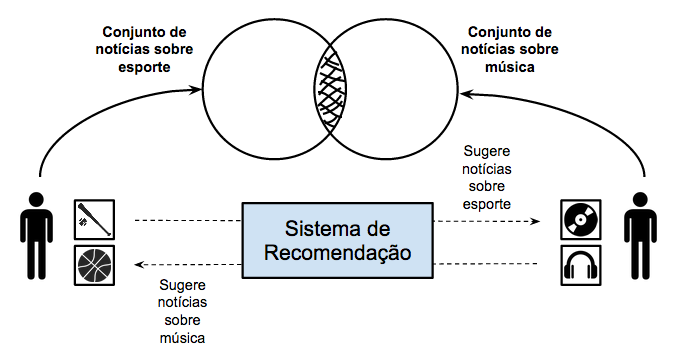
\includegraphics[width=120mm]{img/story.png}
\caption{Ilustração do caso de dois usuários em um portal de notícias com um SR.}
\label{fig:story}
\end{figure}

Assim, faz-se interessante o desenvolvimento de estratégias que permitam melhorar a característica de serendipidade de SR e, especificamente neste trabalho, estratégias de biclusterização, que permitem a análise de correlações parciais entre os atributos descritivos de dados que comporão um grupo de objetos similares, são consideradas candidatas a suprir essa lacuna \cite{Hartigan1972,Mirkin1996,Madeira2004}.

\section{Apresentação do Problema de Recomendação}

Há diferentes tipos de recomendação que podem ser considerados (Seção~\ref{sec:sr}). Aqui, o problema de recomendação com base em conteúdo é apresentado, fazendo uma adaptação de \citeonline{Adomavicius2005}.

Seja um conjunto de usuários $U = \{ u_1, u_2, \dots, u_n, \dots u_N \}$, um conjunto de itens ${\cal I} = \{ I_1, I_2, \dots, I_m, \dots, I_M \}$ e o histórico $h_{u_n,I_m} \in {\cal H}$ indicando se o usuário $u_n$ acessou o item $I_m$.
O problema de recomendação, com base no conteúdo, pode ser visto como a definição de uma função de similaridade entre itens $s: I \rightarrow I \times I$ para aproximar uma função $l: {\cal H}_u, s \rightarrow L_u$, onde ${\cal H}_u$ é o subconjunto que representa o histórico de itens que $u$ acessou, e $L_u$ é a lista de recomendações de itens direcionadas à $u$.

% Achei estranho não ter uma referência aqui. Geralmente definições de conceitos já maduros devem vir de referências importantes. 

A idéia é que a lista de recomendações $L_u$ permita a ocorrência de \textit{serendipidade}, incluindo um fator de ponderação na função de similaridade $s$, que considere similaridades parciais.

\section{Apresentação do contexto de Biclusterização}

O problema de biclusterização, em Mineração de Dados, é referente ao processo de clusterização simultâneo de linhas e colunas em um conjunto de dados.
Capaz de agrupar objetos similares desse conjunto de dados, considerando seus atributos que apresentem alta correlação, formando grupos de objetos e atributos, simultaneamente, chamados de biclusters.
Com maior formalidade, o problema de biclusterização consiste em uma matriz $A$, de dimensão $N \times M$, um conjunto de linhas (objetos) $X = \{ x_1, \dots, x_N \}$ e um conjunto de colunas (atributos) $Y = \{ y_1, \dots, y_M \}$, em que $a_{nm}$, geralmente um número real, e representa a relação entre a linha $x_n$ e a coluna $y_m$ \cite{Franca2010,Mirkin1996,Madeira2004}.

O problema de biclusterização pode ser ilustrado na Figura~\ref{fig:bicluster-exp}, onde se tem um conjunto de dados que possui objetos $x_1, x_2, x_3, x_4, x_5$ e $x_6$ que são representados pelos atributos $y_1, y_2, y_3, y_4, y_5$ e $y_6$, onde $N,M = 6$.
Na Figura~\ref{fig:bicluster-exp} também estão ilustrados dois biclusters hipotéticos: o primeiro formado pelos objetos $x_5$ e $x_6$ e todos os atributos ($y_1, \dots, y_6$), representando um bicluster com \textit{modelo global}; e o segundo formado pelos objetos $x_2, x_3, x_4$ e $x_5$ e atributos $y_4, y_5$ e $y_6$, representando um bicluster com \textit{modelo local}, que leva em consideração apenas um subconjunto dos atributos.

\begin{figure}[h]
\centering
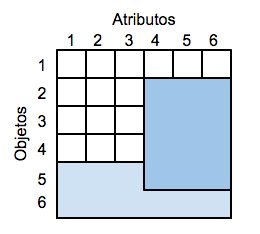
\includegraphics[width=80mm]{img/bicluster.png}
\caption{Conjunto de dados com dois biclusters encontrados.}
\label{fig:bicluster-exp}
\end{figure}

% Apresentar em linhas gerais a possibilidade de implementar bicluterização usando a alternativa de essemble.

% PELO QUE ENTENDI ESSA PARTE DE ESSEMBLE NAO VAI SER TRATADA NA QUALI. MAS NAO ESQUEÇA QUE ELA DEVERÁ ENTRAR NO SEU TRABALHO. ENTAO, TANTO ESSEMBLE QUANTO MARKOV DEVEM SER CITADAS NA PROPOSTA COMO POSSIBILIDADES DE USO E PARA QUE.

\section{Hipótese}

A falta de \textit{serendipidade} nas recomendações é um problema para SRs baseados em conteúdo.
Biclusterização é uma técnica capaz de expandir as possibilidades de formação de clusters, levando em consideração a análise de subconjuntos de atributos para análise de similaridade entre dados a serem considerados como pertencentes a um cluster, ou bicluster.
A possibilidade de considerar a análise de subconjuntos de atributos pode levar à descoberta de objetos similares, que não são necessariamente similares, quando todo o conjunto de atributos é considerado.
Sendo assim, a hipótese formulada nesse projeto é que considerar similaridades parciais entre itens a serem recomendados pode melhorar a serendipidade das recomendações e, uma forma de implementar essa estratégia em SRs, seria por meio da aplicação de algoritmos de biclusterização sobre o conjunto de itens a serem recomendados.

\section{Objetivos}

O objetivo geral desse trabalho é amenizar a dificuldade de oferecer recomendações com \textit{serendipidade} em SRs que se baseiam no conteúdo textual.
Esse objetivo deverá ser atingido por meio da aplicação de técnicas de clusterização de texto, em particular pela aplicação de algoritmos de biclusterização.

%Lucas, leia esse parágrafo abaixo com cuidado e reflita se é isso mesmo.
A clusterização, nesse contexto, deve atuar como estratégia de organização do conteúdo textual, agrupando itens em biclusters.
Sendo que a partir da observação dos interesses do usuário e dos biclusters à que estes itens pertencem, é possível organizar a lista recomendação com itens desses biclusters que esse usuário ainda não interagiu.

Assim, com o intuito de melhor definir o contexto de estudo neste trabalho, foram estabelecidos os seguintes objetivos específicos:

\begin{itemize}
 \item Levantamento do referencial teórico de SRs.
 \begin{itemize}
  \item Levantamento do estado da arte sobre o uso de aprendizado de máquina na implementação de SRs baseados em conteúdo textual.
 \end{itemize}
 \item Levantamento do referencial teórico sobre Biclusterização e Mineração de Texto.
 \item Construção de um corpus de itens textuais e um conjunto de dados de recomendação.
 \item Implementação e teste dos algoritmos de biclusterização sobre o corpus construído.
 \item Modelagem do problema de recomendação baseado em conteúdo considerando a existência de biclusters de itens.
 \item Análise da viabilidade da modelagem proposta frente ao conjunto de dados de recomendação e frente a análise qualitativa do alcance da serendipidade.
 % \item estudo das técnicas de essemble aplicadas a texto
\end{itemize}

\section{Metodologia}

A análise exploratória da literatura especilizada foi escolhida como estratégia para a aquisição de conhecimento sobre a área de SR, biclusterização e mineração de textos.
Já para o levantamento do estado da arte em SRs baseados em conteúdo textual e sobre a aplicação de técnicas de Aprendizado de Máquina, mais especificamente clustering, em SRs baseados em conteúdo textual, optou-se por aplicar a técnica de construção de revisões sistemáticas.
A Revisão Sistemática (RS) é um tipo de revisão bibliográfica documentada, na qual cada passo da pesquisa é registrado seguindo critérios rigorosos, e portanto permitindo facilmente a auditoria e reprodução da pesquisa.
Segundo \citeonline{Kitchenham2004}, a RS é um meio de avaliar, identificar e interpretar todas as pesquisas relevantes disponíveis em uma determinada área com base em questões de pesquisa.
A revisão sistemas que relaciona Aprendizado de Máquina e SRs se faz útil uma vez que a aplicação de Biclusterização como estratégia de resolução do problema é o núcleo deste projeto.

A fim de permitir os testes e validações sobre a modelagem a ser proposta para verificação da hipótese formulada neste projeto, faz-se necessário a definição de um contexto para realização de uma prova de conceito.
Assim, foi escolhido usar o conteúdo referente à notícias publicadas no Portal iG\footnote{http://ig.com.br/}.
Trata-se de um portal de notícias brasileiro muito conhecido, com um volume de notícias bastante grande e com alguma estrutura de classificação de notícias já existente.
Essas características conferem liberdade para a configuração de experimentos de diferentes naturezas, como experimentos considerando determinadas classes de notícias, tipos de notícias ou datas de publicação das notícias.

A partir do conteúdo de notícias do Portal iG deve ser construído um corpus de dados textuais, categorizados de acordo com as categorias já usadas no referido portal.
Todo o conteúdo do corpus deve passar por rotinas de pré-processamento comuns na área de Mineração de Texto: \textit{tokenização}, filtragem de \textit{stopwords}, remoção de sufixos (\textit{stemming}), representação da relação ``termos $\times$ documentos'' usando estratégias de frequência relativa de termos e \textit{n-gramas}.

%Leia com muito cuidado e veja se faz sentido. MUITO CUIDADO.ALTERE O QUE FOR NECESSÄRIOS TAMBÉM COM MUITO CUIDADO.
Também, o Portal iG possui informações históricas e anônimas referentes ao registro de navegação de usuários.
Esse registro permite a construção de um conjunto de dados de preferências, que pode ser usado para realização de \textit{testes offline} entre recomendações oferecidas pela abordagem proposta e a navegação real realizada por um conjunto de usuários, utilizando métricas como precisão e revocação \cite{Jannach2011}.

Os resultados da aplicação dos algoritmos de análise de texto via biclusterização deverão ser validados fazendo a técnicas de avaliação internas, para a verificação da consistência dos biclusters encontrados \cite{Santamaria2007}, e externas \cite{Hochreiter2010}, avaliando o quanto os biclusters encontrados estão em consenso com as classes de notícias \cite{Hochreiter2010}.
% essa parte aqui ficou bem frágil. 
% Os algoritmos de análise de texto via biclusterização deverão ser validados antes de serem aplicados ao corpus criado.
% Para isso, conjuntos de dados de referência para biclusterização e para clusterização de texto deverão ser usados.
% Uma vez alcançada a análise dos textos via biclusterização, o modelo de uso dos biclusters em um contexto de recomendação deverá ser delineado e analisado.
% A análise deverá estar baseando tanto em comparações com o conjunto de dados de recomendação do portal iG quando por análise qualitativa do alcance da serendipidade. 

% Veja se você se sente seguro com isso.
Em tempo, estuda-se a possibilidade de aplicar técnicas de \textit{ensemble} com algoritmos clássicos de clusterização a fim de substituir o uso de algoritmos de biclusterização na análise da correlação parcial dos atributos descritivos dos itens sob recomendação. Ainda, modelos escondidos de Markov podem ser aplicados na modelagem da recomendação sobre o conjunto de dados de recomendação a fim de gerar instâncias de comparação para avaliação da análise proposta neste projeto.

% essa parte você coloca no capítulo 4. Na proposta. Em algum lugar você vai dizer o que já foi feito então você pode dizer que acessou esse material na análise exploratória. Aqui é para falar qual é a metodologia, e não relatar o que já foi feito.

%Para conhecer a área de Sistemas de Recomendação foi realizado um levantamento do referencial teórico através da análise exploratória de livros e artigos do tipo revisão bibliográfica \cite{Adomavicius2005,Lops2011,Ricci2011,Ricci22011,Jannach2011,Burke2002}, o que permitiu, em seguida, o aprofundamento na área de SRs.
%Para o aprofundamento na área de SRs, foi realizada uma Revisão Sistemática de SRs baseados em conteúdo textual.
%Também foi realizado um levantamento do referencial teórico, através da análise exploratória de livros e artigos do tipo revisão bibliográfica, na área de Mineração de Dados \cite{Berry2010,Feldman2006,Miner2012,Hotho2005,Weiss2010}, para que fosse possível realizar a análise e estruturação do conteúdo não-estruturado, presentes nas notícias.

%Isso tudo tem que vir no capitulo da propsota, como eu disse, aqui é não é um momento de relatar atividades realizadas.
% Sendo assim, com a extração das notícias do portal iG\footnote{http://ig.com.br/} através de um \textit{web crawler} utilizando a linguagem python\footnote{https://www.python.org/}, foi possível construir o corpus iG (Subseção~\ref{subsec:corpusig}) de notícias.
%As notícias foram capturadas a partir de uma página de início, fornecida para o \textit{web crawler}, que era selecionada a fim de equalizar a distribuição de notícias por ano e por assunto. Este trabalho também conta com uma base de cliques em notícias (Subseção~\ref{subsec:basecliquesig}), doada pelo portal de notícias iG.

%idem
%Para aplicação dos algoritmos de biclusterização, foi realizado um levantamento do referencial teórico, através da análise exploratória de livros, artigos do tipo revisão bibliográfica e artigos que se referem à criação dos algoritmos \cite{Cheng2000,Tanay2005,Madeira2004,Santamaria2007,Kluger2003,Prelic2006}.

%Para gerar conhecimento do corpus iG, serão aplicados algoritmos de Biclusterização que estão sendo implementados\footnote{https://github.com/lucasbrunialti/biclustering-experiments} nos textos das notícias processados e representados por diversas estratégias (TF-IDF, TF-IDF normalizado e n-gramas). Assim, será possível avaliar o resultado dos algoritmos utilizando a base de dados de cliques iG.

\section{Organização do documento}

Este documento é composto por quatro capítulos incluindo esta introdução. No Capítulo 2 conceitos fundamentais necessários para a compreensão deste projeto são apresentados, incluindo conceitos sobre SRs, biclusterização e mineração de texto; o Capítulo 3 apresenta uma revisão sistemática sobre aprendizado de máquina aplicado à SRs baseados em conteúdo; por fim, o capítulo 4 apresenta em detalhes a proposta desse projeto de mestrado, um relato sobre os resultados já obtidos e o cronograma que guia a realização das próximas atividades.

\chapter{Conceitos Fundamentais}

Este capítulo introduz os conceitos fundamentais para o entendimento dessa dissertação, fazendo um apanhado dos conceitos na área de Sistemas de Recomendação (seção~\ref{sec:sr}), Biclusterização (seção~\ref{sec:bicl}) e Mineração de Texto (seção~\ref{sec:mintexto}).

\section{Sistemas de Recomendação}
\label{sec:sr}

% provavelmente vou ter que fazer o bib de tese-chap2: http://tampub.uta.fi/bitstream/handle/10024/95965/978-951-44-9551-9.pdf
A grande maioria das pessoas que usam a Internet muito provavelmente já interagiram com algum Sistema de Recomendação (SR), por isso, o seu conceito é intuitivo.
Porém, por ser uma área relativamente nova \cite{Lops2011}, muitos autores não usam uma definicão que reflete a realidade dos SRs, isso acontece por ser uma área relativamente nova que teve um crescimento muito grande nos últimos anos \cite{Leino2014}.

\citeonline{Resnick1997}, quem criou o termo Sistemas de Recomendação (tese-chap2) \cite{Neumann2007}, argumentam que Sistemas de Recomendação servem para nos ajudar em processos de tomada de decisão do nosso dia-a-dia, como quais itens comprar, quais músicas ouvir, ou quais notícias ler.
Além disso, \citeonline{Resnick1997} provê uma taxonomia para definição de Sistemas de Recomendação:
\begin{itemize}
  \item Conteúdo recomendado: os itens que são recomendados pelo Sistema de Recomendação, ex: produtos, músicas, notícias e/ou etc.
  \item Entrada dos usuários: as interações que os usuários realizam com os itens são a entrada para um SR, estas podem ser implícitas (ex: o usuário $x$ leu a notícia $y$) ou explícitas (ex: o usuário $x$ classificou o filme $y$ como $5$ estrelas).
  \item Target of recommendation: os itens recomendados podem ser diretamente para um usuário (personalizado), direcionados para um grupo de usuários ou todos os usuários (não-personalizado).
  \item Técnicas para recomendação (agregações): qual as estratégias e os algoritmos que os SRs usam para criar recomendações.
  \item Uso das recomendações: trata-se de como mostrar as recomendações para os usuários, ex: filtrando recomendações negativas, ordenando pelo fator numérico, etc.
\end{itemize}

Porém, definições mais recentes \cite{Burke2002,Burke2007}, descrevem SRs como qualquer sistema que produz recomendações personalizadas ou tem o efeito de guiar um usuário de modo personalizado, mostrando itens que possam ser interessantes para este usuário, dentro de uma grande quantidade de opções.
Isso faz com que SRs que provêm recomendações não personalizadas deixem de adequar com a definição de SR.
É provável que isso se deve ao fato que das estratégias usadas atualmente, que têm o foco de produzir recomendações personalizadas.

Formalmente, \citeonline{Burke2002,Burke2007} define SRs como um conjunto de itens $I$  que podem ser recomendados e um conjunto de usuários $U$ que as preferências são conhecidas, um usuário $u$ pra o qual as recomendações são geradas, e algum item $i$ que queremos predizer a preferência para $u$.
\citeonline{Adomavicius2005} extende a definição com uma função de utilidade $f$ que mede o quão útil é o item $i$ para o usuário $u$: $f: I \times U \rightarrow R$, em que $R = \{ r_{u_1,i_1}, r_{u_1,i_2}, \dots, r_{u_1,i_m}, \dots, r_{u_n,i_1}, \dots, r_{u_n,i_m} \}$ é um conjunto ordenado com valores faltantes, sendo $r_{u_i,i_j}$ um inteiro ou real que representa a interação do usuário $u_i$ no item $i_j$.
No entanto, existem tipos de SRs que não estimam $f$ completamente, podendo otimizar funções auxiliares para gerar as recomendações à um usuário $u$ \cite{Lops2011}.

Em síntese, um Sistema de Recomendação tem a função de auxiliar os usuários de uma aplicação à interagir com itens, provendo sugestões de quais itens interagir, baseando-se no histórico de interações desses usuários com esses itens.

 \subsection{Tipos de Sistemas de Recomendação}
 \label{subsec:tipossr}

Para estimar $f$ e chegar no conjunto ordenado $R$ existem diversas estratégias, daí surgem os tipos de SRs.
Os tipos de SRs diferem quanto ao domínio, informações usadas para recomendação, algoritmos \cite{Feldman2006}, e principalmente nas propriedades em que cada tipo se destaca.

% Não sei se coloco a taxonomia tradicional, ou se coloco essa, handbook-1 diz que é clássica, podem burke de 2002 para 2007 muda a taxonomia, enquanto isso, Adomavicius usa a tradicional e o livro usa a tradicional + baseado em conhecimento
\citeonline{Burke2002,Burke2007} provê uma taxonomia já considerada clássica \citeonline{Lops2011}, que categoriza os SRs em cinco diferentes tipos:
\begin{itemize}
 \item \textit{Filtragem colaborativo}, o primeiro tipo de SR que foi implementado \cite{Resnick1997}, tem como idéia básica encontrar outros usuários $u_{1,\dots,n}$ em $U$, sendo $n < |U|$ e não necessariamente em ordem, com preferências semelhantes à $u$, e então recomendar itens que $u_{1,\dots,n}$ interagiram e que $u$ ainda não interagiu, estabelecendo alguma métrica para estimar $f$. Medidas geralmente usadas incluem \textit{Correlação de Pearson} e \textit{Similaridade dos Cossenos}, também são usados técnicas para redução de dimensionalidade, como \textit{Decomposição de Valores Singulares} e \textit{Fatorização de Matriz} \cite{Jannach2011}.
 \item \textit{Baseado em conteúdo}, é um dos tipos de SR que otimiza funções auxiliares à $f$. Descreve os itens por características possibilitando o uso de medidas de similaridade entre itens. Então, com as interações dos usuários de $U$ sob itens em $I$, é construído um perfil de interesses para cada usuário. As recomendações são feitas a partir da combinação do perfil de interesses de um usuário $u$ com os itens em $I$ que $u$ ainda não interagiu. Neste caso são usadas técnicas de Recuperação de Informação \cite{Jannach2011} para representar os itens e calcular similaridades entre itens, assim como técnicas de Aprendizado de Máquina Supervisionado e não-supervisionado \cite{Jannach2011,Burke2002}.
 % \item Demográfico, considera atributos demográficos de cada usuário, estimando $f$ a partir dessas informações. Neste tipo também são usadas técnicas de Aprendizado de Máquina Supervisionado para classificar usuários em diferentes classes demográficas.%constrói recomendações personalizadas com base no perfil demográfico de usuários
 \item \textit{Baseado em Conhecimento}, tem o intuito de sugerir itens, de forma personalizada, baseando-se nas necessidades ou regras estabelecidas por um usuário $u$ e nas características dos itens em $I$. São estabelecidas medidas de similaridade para estimar o quanto as necessidades do usuário match as recomendações \cite{Jannach2011,Lops2011,Burke2007}.
 \item \textit{Híbrido}, é capaz de combinar as vantagens de cada tipo de SR descrito para suprir as limitações associadas à cada tipo. A dificuldade esta em como combinar as diferentes técnicas de cada algoritmo \cite{Jannach2011,Burke2007}. \citeonline{Burke2007} identificou 7 tipos de SRs Híbridos em uma revisão da literatura: Pesagem, atribui um peso para cada algoritmo; Switching, seleciona um dos algoritmos (ou tipos); Mixed, recomendações são mostradas em conjunto; Combinação de características, diferentes fontes são combinadas em apenas um algoritmo; Feature Augumentation, uma técnica é usada para computar características que servem de entrada para outra técnica; Cascade, é atribuído um grau de prioridade para cada algoritmo; Meta-level, uma técnica gera um modelo, que é usado como entrada para outras técnicas.
\end{itemize}

 \subsubsection{Vantagens e desvantagens}
 \label{subsubsec:lim}

Cada um dos tipos de SRs descritos possuem algumas limitações independentes se comparados com os outros tipos ou não.
Em \citeonline{Jannach2011,Adomavicius2005,Burke2002,Lops2011} são nomeadas os problemas no desenvolvimento de SRs de \textit{novo usuário} (\textit{user cold-start}), \textit{novo item} (\textit{item cold-start}), \textit{esparsidade}, \textit{sobre-especialização} e \textit{análise de conteúdo limitada} referentes aos SRs.

Os problemas de \textit{novo usuário} e \textit{novo item} são similares, basicamente, enquanto o primeiro se trata da dificuldade de gerar recomendações para novos usuários, o segundo se trata de gerar recomendações para novos itens.
O problema de \textit{novo usuário} esta presente como uma desvantagem nos SRs de filtragem colaborativa e baseado em conteúdo, pois o SR não conhece as preferências dos novos usuários, tendo dificuldade de construir um modelo que tem como base essas preferências.
Já o problema de \textit{novo item} é considerado uma vantagem para os SRs baseados em conteúdo, enquanto uma desvantagem para os SRs baseados em filtragem colaborativa.
Como a filtragem colaborativa se baseia apenas nas interações de usuários em itens, um item novo, que não teve ou teve poucas interações, não será recomendado, diferentemente do SR baseado em conteúdo, que leva em consideração a representação do item para construir recomendações.

Contrariamente, o problema de \textit{sobre-especialização} é uma vantagem para os SRs de filtragem colaborativa e uma desvantagem para os SRs baseados em conteúdo.
A \textit{sobre-especialização} diz respeito ao problema de sugerir apenas itens previsíveis para o usuário, por exemplo, se o usuário viu notícias apenas de esporte, ele já espera receber sugestões de notícias de esporte, porém este usuário muito provavelmente pode gostar de ler notícias de outras categorias.
A capacidade do SR de sugerir notícias imprevisíveis é chamado de \textit{serendipidade} \cite{Jannach2011,Lops2011}.
SRs baseados em conteúdo sofrem desse problema pois combina o perfil de preferências de um usuário com os itens em $I$, restrigindo o espaço de busca para realizar a sugestão de itens.
Enquanto isso, os SRs baseados em filtragem colaborativa são capazes de oferecer sugestões úteis e serendipitas, pois são capazes de ampliar o espaço de busca através da estratégia de sugerir itens que usuários semelhantes à $u$ interagiram e que $u$ ainda não interagiu.

Os SRs baseados em filtragem colaborativa são os únicos que sofrem do problema de \textit{esparsidade}, que é o fato de usuários interagirem com apenas um pequeno subconjunto do conjunto de itens, tornando a matriz de interações ou preferências ($U \times I$) esparsa.
Isso faz com que aumente a necessidade de ter uma grande quantidade de usuários, pois este tipo de SR necessita de intersecções nas interações de itens por usuários, para que seja possível encontrar usuários similares a um dado usuário.

Assim como os SRs de filtragem colaborativa, os SRs baseados em conteúdo sofrem de um problema único, que é a \textit{análise de conteúdo limitada}.
Este problema se refere à representação dos itens, que tem de ser suficiente para discriminá-los \cite{Lops2011}.
Em SRs baseados em conteúdo é comum ter que limitar a representação de itens, tanto pelo número de características quanto pela modelagem.
Por exemplo, no contexto de notícias na web, se a representação for um vetor com o número de ocorrências de cada palavra, perdemos a relação entre as palavras, e também todo o conteúdo que não é texto, como imagens, vídeos, etc.

 \subsection{Avaliação da Recomendação}
 \label{subsec:evalsr}

Diferentes técnicas foram mostradas e uma variedade de problemas relacionados à essas técnicas, mas como avaliar se uma estratégia adotada no desenvolvimento realmente é efetiva?
SRs podem ser avaliados através de \textit{experimentos online}, que podem descobrir a real influência do SR no comportamento do usuário, e \textit{experimentos offline}, que estimam o erro de predição e simulam o comportamento do usuário no SR usando um conjunto de dados \cite{Ricci22011}.

Para experimentos online podem ser estabelecidas variáveis através da captura implícita ou explícita do comportamento, como satisfação do usuário e taxa de cliques (\textit{click-through rate} - CTR).
Uma das maneiras para realizar esse tipo de experimento é por meio de testes A/B \cite{Jannach2011}, em que cada usuário, ao interagir com o SR, recebe um tratamento diferente aleatóriamente, dentro dos possíveis tratamentos estabelecidos pelo experimento.
Assim, é possível dizer, por exemplo, a influência de um novo componente no SR no comportamento dos usuários.

Tradicionalmente, SRs são avaliados através de experimentos offline \cite{Jannach2011}.
Por serem simples, esses tipos de experimentos podem ser usados para para selecionar algoritmos, no entanto, \citeonline{Ricci22011} argumentam que não é possível medir diretamente a influência das recomendações no comportamento dos usuários.
Para simular o comportamento do usuário em um SR usando um conjunto de dados, são estabelecidos dois subconjunto das interações de $u$ aleatoriamente ($\{ r_{u,i_4}, r_{u,i_3}, \dots \}$), um para treinamento dos modelos $\text{conj treino}_u$ e outro para teste $\text{conj teste}_u$.
Assim é possível adotar estratégias semelhantemente com às adotadas em Aprendizado de Máquina, como \textit{matriz de confusão}, \textit{precisão}, \textit{revocação}, \textit{f1-score}, \textit{cross-validation} e etc.
A técnica de \textit{matriz de confusão} é possível ser usada em \textit{experimentos online} e \textit{offline}, da seguinte maneira: se o usuário gostar do item sugerido à ele, é considerada uma predição correta (verdadeiro positivo); se o usuário não solicita preferência pela sugestão ou se não existe informações da preferência do usuário para esta sugestão, será considerada uma predição errada (falso positivo); contrariamente, se o SR não fazer essas sugestões, é considerada uma emissão correta (verdadeiro negativo); por fim, se o SR não sugerir itens que o usuário tem preferência, é consuderada uma predição errada (falso negativo).

Uma das métricas mais comuns usadas para \textit{experimentos offline} é o \textit{erro absoluto médio} (\textit{Mean Absolute Error} - MAE) e \textit{raiz do erro quadrático médio} (\textit{Root Mean Squared Error} - RMSE) \cite{Jannach2011}, o qual foi usado como métrica para a competição Netflix Prize\footnote{\textit{http://www.netflixprize.com/}}, que teve grande repercursão na academia e na indústria. A defição formal das métricas MAE e RMSE são descritas nas equações~\ref{eq:mae} e~\ref{eq:rmse}, respectivamente.

\begin{equation}
\label{eq:mae}
MAE = \sum_{u \in U} \frac{\sum_{i \in \text{conj teste}_u} |f(u,i) - r_{u,i}|}{|\text{conj teste}_u|}
\end{equation}

\begin{equation}
\label{eq:rmse}
RMSE = \sum_{u \in U} \sqrt{\frac{\sum_{i \in \text{conj teste}_u} (f(u,i) - r_{u,i}^2}{|\text{conj teste}_u|}}
\end{equation}

A métrica MAE computa o erro médio entre as predições feitas pelo SR ($f(u,i)$) e os valores reais das preferências dos usuários ($r_{u,i}$) para todos os usuários em $U$, enquanto o RMSE amplifica erros grandes, pois eleva o mesmo ao quadrado. Essas métricas são usadas para valores reais, ou seja, $r_{u,i} \in [0,1]$, por exemplo.

Para valores binários de $r_{u,i}$ ou quando deseja-se prever o número de recomendações relevantes para um usuário $u$, são usadas as métricas \textit{precisão} e \textit{revocação} \cite{Jannach2011}.

Para medir a \textit{serendipidade} das recomendações, \citeonline{Ricci22011} propõem uma estratégia: estabelecer uma medida de distância entre itens e rotular os itens com menor distância entre si como ausentes de \textit{serendipidade}, assim, algoritmos que evitem esses itens, serão considerados superiores.

\section{Biclusterização}
\label{sec:bicl}

Técnicas e algoritmos de biclusterização são usadas, principalmente, no contexto de expressão genética.
No entanto, algoritmos de biclusterização se fazem útil quando se deseja encontrar \textit{modelos locais}.
Ou seja, enquanto algoritmos de clusterização têm o intuito de encontrar \textit{modelos globais}, que geram grupos de dados levando em consideração todas as características, algoritmos de biclusterização geram grupos de dados em que as características tem alta correlação \cite{Madeira2004}.

Para a descrição do problema formal de biclusterização usa-se a seguinte definição \cite{Madeira2004}: uma matriz $A$, $n \times m$, um conjunto de linhas $X = \{ x_1, \dots, x_n \}$ e um conjunto de colunas $Y = \{ y_1, \dots, y_m \}$, em que $a_{ij}$, geralmente um número real, e representa a relação entre a linha $x_i$ e a coluna $y_j$.
O problema de biclusterização é encontrar biclusters, que são submatrizes de $A$, denotados por $A_{IJ}$, em que $I \subseteq X$ e $J \subseteq Y$.
Assim, o bicluster $A_{IJ}$ é um grupo dos exemplos em $I$, perante as características com alta correlação $J$.

\subsection{Tipos de biclusters}
\label{sec:tiposbic}

<<<<<<< HEAD
    Como a definição de bicluster não inclui uma prévia estrutura da matriz $A$ e dos biclusters $A_{IJ}$, diversos algoritmos propostos na literatura diferem quanto ao tipo de bicluster que são capazes de encontrar. Uma taxonomia dos tipos de biclusters é proposta por \citeonline{Madeira2004}:
     \begin{itemize}
      \item \textit{Biclusters com valores constantes}, se trata de biclusters em que todos os valores de $A_{IJ}$ são constantes: $a_{ij} = \mu, \forall i,j \in I,J$, onde $\mu$ é um valor constante dentro de $A_{IJ}$. Porém, em conjuntos de dados reais, esses biclusters estão presentes com algum tipo de ruído $\mu + \eta_{ij}$, onde $\eta_{ij}$ é o ruído associado com os valures de $\mu$ e $a_{ij}$ \cite{Madeira2004}.
      \item \textit{Biclusters com valores constantes nas linhas ou colunas}, se trata de biclusters com valores constantes nas linhas: $a_{ij} = \mu + \alpha_i, \forall i,j \in I,J$ ou $a_{ij} = \mu \cdot \alpha_i, \forall i,j \in I,J$, onde $\alpha_i$ é um fator aditivo ou multiplicativo para cada linha; ou ainda biclusters com valores constantes nas colunas: $a_{ij} = \mu + \beta_j, \forall i,j \in I,J$ ou $a_{ij} = \mu \cdot \beta_j, \forall i,j \in I,J$, onde $\beta_j$ é um fator aditivo ou multiplicativo para cada coluna \cite{Madeira2004}.
      \item \textit{Biclusters com valores coerentes}, em que são considerados valores próximos entre si (coerentes) para definição de um bicluster: $a_{ij} = \mu + \alpha_i + \beta_j, \forall i,j \in I,J$, ou $a_{ij} = \mu' \cdot \alpha_i' \cdot \beta_j', \forall i,j \in I,J$, sendo que se $\mu = \log \mu'\implies \alpha_i = \alpha_i', \beta_j = \beta_j'$ \cite{Madeira2004}.
      \item \textit{Biclusters com evoluções coerentes}, têm seus valores com evoluções coerentes, por exemplo, um bicluster com $a_{i4} \leq a_{i3} \leq a_{i2} \leq a_{i1}$ tem valores com evolução coerente na coluna \cite{Madeira2004}. Seus valores podem ser gerados por uma função geradora de valores com evolução coerente $a_{ij} = g(a_{ij}), \forall i,j \in I,J$, sendo $g(\cdot)$ não linear e não constante, para que o tipo de bicluster não seja classificado nos casos anteriores.
     \end{itemize}
    
    Os biclusters também se diferem quanto a sua estrutura, cada algoritmo faz uma suposição da estrutura de biclusters que é capaz de encontrar. A Figura~\ref{fig:bicstruct} sumariza as diferentes estruturas de biclusters, com as linhas e colunas ordenadas, para permitir a visualização dos biclusters por meio do mapa de calor dos valores de $A$.

    \begin{figure}[h]
        % \captionsetup[subfigure]{labelformat=simple}
        \centering
        \begin{subfigure}[b]{0.3\textwidth}
                
\includegraphics[width=30mm]{img/a-bic-struct.png}
                \caption{Bicluster único}
                \label{fig:bicstruct-a}
        \end{subfigure}
        ~
        \centering
        \begin{subfigure}[b]{0.3\textwidth}
                
\includegraphics[width=30mm]{img/b-bic-struct.png}
                \caption{Biclusters com linhas e colunas exclusivas}
                \label{fig:bicstruct-b}
        \end{subfigure}
        ~
        \centering
        \begin{subfigure}[b]{0.3\textwidth}
                
\includegraphics[width=30mm]{img/c-bic-struct.png}
                \caption{Biclusters com estrutura de tabuleiro de xadrez}
                \label{fig:bicstruct-c}
        \end{subfigure}
        ~
        \centering
        \begin{subfigure}[b]{0.3\textwidth}
                
\includegraphics[width=30mm]{img/d-bic-struct.png}
                \caption{Biclusters com linhas exclusivas}
                \label{fig:bicstruct-d}
        \end{subfigure}
        ~
        \centering
        \begin{subfigure}[b]{0.3\textwidth}
                
\includegraphics[width=30mm]{img/e-bic-struct.png}
                \caption{Biclusters com colunas exclusivas}
                \label{fig:bicstruct-e}
        \end{subfigure}
        ~
        \centering
        \begin{subfigure}[b]{0.3\textwidth}
                
\includegraphics[width=30mm]{img/f-bic-struct.png}
                \caption{Biclusters sem sobreposição com estrutura em árvore}
                \label{fig:bicstruct-f}
        \end{subfigure}
        ~
        \centering
        \begin{subfigure}[b]{0.3\textwidth}
                
\includegraphics[width=30mm]{img/g-bic-struct.png}
                \caption{Biclusters sem sobreposição e não exclusivos}
                \label{fig:bicstruct-g}
        \end{subfigure}
        ~
        \centering
        \begin{subfigure}[b]{0.3\textwidth}
                
\includegraphics[width=30mm]{img/h-bic-struct.png}
                \caption{Biclusters com sobreposição com estrutura hierarquica}
                \label{fig:bicstruct-h}
        \end{subfigure}
        ~
        \centering
        \begin{subfigure}[b]{0.3\textwidth}
                
\includegraphics[width=30mm]{img/i-bic-struct.png}
                \caption{Biclusters com sobreposição arbitrariamente posicionados}
                \label{fig:bicstruct-i}
        \end{subfigure}
        \caption{Diferentes estruturas de biclusters, quadrados com cores sólidas representam biclusters} %(Adaptado de \cite{Madeira2004})}  % LUCAS, RETIREI ISSO 
        \label{fig:bicstruct}
    \end{figure}
    
    \subsection{Algoritmos para biclusterização}
=======
Como a definição de bicluster não inclui uma prévia estrutura da matriz $A$ e dos biclusters $A_{IJ}$, diversos algoritmos propostos na literatura diferem quanto ao tipo de bicluster que são capazes de encontrar. Uma taxonomia dos tipos de biclusters é proposta por \citeonline{Madeira2004}:
 \begin{itemize}
  \item \textit{Biclusters com valores constantes}, se trata de biclusters em que todos os valores de $A_{IJ}$ são constantes: $a_{ij} = \mu, \forall i,j \in I,J$, onde $\mu$ é um valor constante dentro de $A_{IJ}$. Porém, em conjuntos de dados reais, esses biclusters estão presentes com algum tipo de ruído $\mu + \eta_{ij}$, onde $\eta_{ij}$ é o ruído associado com os valures de $\mu$ e $a_{ij}$ \cite{Madeira2004}.
  \item \textit{Biclusters com valores constantes nas linhas ou colunas}, se trata de biclusters com valores constantes nas linhas: $a_{ij} = \mu + \alpha_i, \forall i,j \in I,J$ ou $a_{ij} = \mu \cdot \alpha_i, \forall i,j \in I,J$, onde $\alpha_i$ é um fator aditivo ou multiplicativo para cada linha; ou ainda biclusters com valores constantes nas colunas: $a_{ij} = \mu + \beta_j, \forall i,j \in I,J$ ou $a_{ij} = \mu \cdot \beta_j, \forall i,j \in I,J$, onde $\beta_j$ é um fator aditivo ou multiplicativo para cada coluna \cite{Madeira2004}.
  \item \textit{Biclusters com valores coerentes}, em que são considerados valores próximos entre si (coerentes) para definição de um bicluster: $a_{ij} = \mu + \alpha_i + \beta_j, \forall i,j \in I,J$, ou $a_{ij} = \mu' \cdot \alpha_i' \cdot \beta_j', \forall i,j \in I,J$, sendo que se $\mu = \log \mu'\implies \alpha_i = \alpha_i', \beta_j = \beta_j'$ \cite{Madeira2004}.
  \item \textit{Biclusters com evoluções coerentes}, têm seus valores com evoluções coerentes, por exemplo, um bicluster com $a_{i4} \leq a_{i3} \leq a_{i2} \leq a_{i1}$ tem valores com evolução coerente na coluna \cite{Madeira2004}. Seus valores podem ser gerados por uma função geradora de valores com evolução coerente $a_{ij} = g(a_{ij}), \forall i,j \in I,J$, sendo $g(\cdot)$ não linear e não constante, para que o tipo de bicluster não seja classificado nos casos anteriores.
 \end{itemize}
>>>>>>> master

Os biclusters também se diferem quanto a sua estrutura, cada algoritmo faz uma suposição da estrutura de biclusters que é capaz de encontrar. A Figura~\ref{fig:bicstruct} sumariza as diferentes estruturas de biclusters, com as linhas e colunas ordenadas, para permitir a visualização dos biclusters por meio do mapa de calor dos valores de $A$.

\begin{figure}[h]
    % \captionsetup[subfigure]{labelformat=simple}
    \centering
    \begin{subfigure}[b]{0.3\textwidth}
            
\includegraphics[width=30mm]{img/a-bic-struct.png}
            \caption{Bicluster único}
            \label{fig:bicstruct-a}
    \end{subfigure}
    ~
    \centering
    \begin{subfigure}[b]{0.3\textwidth}
            
\includegraphics[width=30mm]{img/b-bic-struct.png}
            \caption{Biclusters com linhas e colunas exclusivas}
            \label{fig:bicstruct-b}
    \end{subfigure}
    ~
    \centering
    \begin{subfigure}[b]{0.3\textwidth}
            
\includegraphics[width=30mm]{img/c-bic-struct.png}
            \caption{Biclusters com estrutura de tabuleiro de xadrez}
            \label{fig:bicstruct-c}
    \end{subfigure}
    ~
    \centering
    \begin{subfigure}[b]{0.3\textwidth}
            
\includegraphics[width=30mm]{img/d-bic-struct.png}
            \caption{Biclusters com linhas exclusivas}
            \label{fig:bicstruct-d}
    \end{subfigure}
    ~
    \centering
    \begin{subfigure}[b]{0.3\textwidth}
            
\includegraphics[width=30mm]{img/e-bic-struct.png}
            \caption{Biclusters com colunas exclusivas}
            \label{fig:bicstruct-e}
    \end{subfigure}
    ~
    \centering
    \begin{subfigure}[b]{0.3\textwidth}
            
\includegraphics[width=30mm]{img/f-bic-struct.png}
            \caption{Biclusters sem sobreposição com estrutura em árvore}
            \label{fig:bicstruct-f}
    \end{subfigure}
    ~
    \centering
    \begin{subfigure}[b]{0.3\textwidth}
            
\includegraphics[width=30mm]{img/g-bic-struct.png}
            \caption{Biclusters sem sobreposição e não exclusivos}
            \label{fig:bicstruct-g}
    \end{subfigure}
    ~
    \centering
    \begin{subfigure}[b]{0.3\textwidth}
            
\includegraphics[width=30mm]{img/h-bic-struct.png}
            \caption{Biclusters com sobreposição com estrutura hierarquica}
            \label{fig:bicstruct-h}
    \end{subfigure}
    ~
    \centering
    \begin{subfigure}[b]{0.3\textwidth}
            
\includegraphics[width=30mm]{img/i-bic-struct.png}
            \caption{Biclusters com sobreposição arbitrariamente posicionados}
            \label{fig:bicstruct-i}
    \end{subfigure}
    \caption{Diferentes estruturas de biclusters, quadrados com cores sólidas representam biclusters (Adaptado de \cite{Madeira2004})}
    \label{fig:bicstruct}
\end{figure}

\subsection{Algoritmos para biclusterização}

Diversos algoritmos para encontrar biclusters, de diferentes tipos e estruturas, foram propostos na literatura \cite{Tanay2005,Madeira2004}.

Um dos mais comuns e simples algoritmos de biclusterização, que encontra biclusters com valores coerentes e estrutura com sobreposição e arbitrariamente posicionados, é o \textit{Coupled Two-way Clustering} (CTWC) \cite{Getz2000}, pois encontra biclusters através da clusterização de características e exemplos (linhas e colunas), separadamente.
O algoritmo de clusterização usado por \cite{Getz2000} foi o \textit{Superparamagnetic Clustering} (SPC), pois é capaz de determinar o número de clusters automaticamente e com uma estratégia de clusterização hierárquica \textit{top-down} é capaz de gerar clusters estáveis \cite{Getz2000}.
O SPC tem como entrada uma matriz de similaridade e um parâmetro temperatura, que controla o quão estáveis serão os clusters que o algoritmo irá gerar.
Assim, o CTWC encontra clusters estáveis de linhas e colunas através do SPC, e iterativamente, performa o SPC novamente nos clusters de linhas e colunas encontrados, mantendo na memória um par do subconjunto de linhas e do subconjunto de colunas (biclusters), assim como os clusters estáveis de linhas e colunas, separadamente.
% O algoritmo se inicia com dois subconjuntos: um para exemplos (linhas) $I = \{ X \}$ e um para características (colunas) $J = \{ Y \}$, então, através do algoritmo de SPC

O algoritmo Cheng e Church \cite{Cheng2000}, é capaz de encontrar o mesmo tipo de bicluster que o algoritmo CTWC, de forma gulosa: biclusters com valores coerentes e estrutura com sobreposição e arbitrariamente posicionados. Este algoritmo esta sendo objeto de estudo desse projeto de mestrado para aplicação em dados textuais.
\citeonline{Cheng2000} introduz o conceito de bicluster no domínio de expressões genéticas. Além disso, para encontrar biclusters, ou $\delta$-biclusters, na matriz $A$, os autores definem o \textit{Resíduo Quadrático Médio} (RQM):
\begin{equation}
\begin{split}
    H_{IJ} = \frac{1}{|I||J|} \displaystyle\sum_{i,j \in I,J} (a_{ij} - a_{iJ} - a_{Ij} + a_{IJ})^2 \\
    H_{iJ} = \frac{1}{|J|} \displaystyle\sum_{j \in J} (a_{ij} - a_{iJ} - a_{Ij} + a_{IJ})^2 \\
    H_{Ij} = \frac{1}{|I|} \displaystyle\sum_{i \in I} (a_{ij} - a_{iJ} - a_{Ij} + a_{IJ})^2
\end{split}
\end{equation}
em que
\begin{equation}
    a_{iJ} = \frac{1}{|J|} \displaystyle\sum_{j \in J} a_{ij},\quad a_{Ij} = \frac{1}{|I|} \displaystyle\sum_{i \in I} a_{ij},\quad a_{IJ} = \frac{1}{|I||J|} \displaystyle\sum_{i,j \in I,J} a_{ij}
\end{equation}
onde $H_{IJ}$ é o RQM de uma submatriz $A_{IJ}$, $H_{iJ}$ o RQM da linha $i$, $H_{Ij}$ o RQM da coluna $j$, $a_{iJ}$ a média dos valores da linha $i$, $a_{Ij}$ a média dos valores da coluna $j$ e $a_{IJ}$ a média dos valores da submatriz $A_{IJ}$, definida pelos subconjuntos $I$ e $J$.

Então, um bicluster um perfeito $A_{IJ}$ teria o RQM $H_{IJ} = 0$, pois $a_{ij} = a_{ij}, \forall i,j \in I,J$, fazendo $a_{iJ} = a_{Ij} = a_{IJ}$. No entanto, se apenas minizar o RQM, um bicluster com apenas um elemento seria perfeito, o que pode não refletir a realidade. Além disso, em conjunto de dados reais existe ruído, podendo esconder o bicluster perfeito.

Para encontrar biclusters, ou $\delta$-biclusters, \citeonline{Cheng2000} fazem uma estratégia gulosa que retira linhas e colunas, visando a minimização do RQM, respeitando um parâmetro $\delta$, que é calibrado pelo usuário. Então, um bicluster é encontrado quando o RQM de uma submatriz $A_{IJ}$ é $H_{IJ} \leq \delta$, para algum $\delta \geq 0$. As etapas de remoções de elementos da matriz são apresentadas nos algoritmos~\ref{algo:cc1} e~\ref{algo:cc2}.

\begin{algorithm}[H]
\label{algo:cc1}
 \KwIn{$A, I, J, \delta$}
 \KwOut{$I,J$ onde $H_{IJ} \leq \delta$}
 \While{$H_{IJ} > \delta$}{
  encontre a linha $l_{max} = \operatorname*{arg\,max}_{i \in I} H_{iJ}$\;
  encontre a coluna $c_{max} = \operatorname*{arg\,max}_{j \in J} H_{Ij}$\;
  \eIf{$l_{max} > c_{max}$}{
   remova $l_{max}$ do subconjunto $I$\;
   }{
   remova $c_{max}$ do subconjunto $J$\;
  }
 }
 \caption{Remove uma linha ou coluna a cada iteração.}
\end{algorithm}

\begin{algorithm}[H]
\label{algo:cc2}
 \KwIn{$A, I, J, \delta, \alpha$}
 \KwOut{$I,J$ onde $H_{IJ} \leq \delta$}
 \While{$H_{IJ} > \delta$}{
  remova $i \in I$ onde $H_{iJ} > \alpha \cdot H_{IJ}$\;
  remova $j \in J$ onde $H_{Ij} > \alpha \cdot H_{IJ}$\;
  encontre a coluna $c_{max} = \operatorname*{arg\,max}_{j \in J} H_{Ij}$\;
  \If{não houve nenhuma remoção}{
   chame o algoritmo~\ref{algo:cc1}
  }
 }
 \caption{Remove múltiplas linhas e colunas de $A$ a cada iteração.}
\end{algorithm}

O algoritmo~\ref{algo:cc2} é usado para acelerar o processo de busca de um $\delta$-bicluster, convergindo mais rapidamente para uma solução quanto maior for o parâmetro $\alpha$, em que $\alpha \geq 0$. Ainda, para amenização do problema de encontrar $\delta$-biclusters perfeitos com apenas um elemento, ou poucos elemento, é utilizado o algoritmo~\ref{algo:cc3}, que adiciona nós sem aumentar o RQM do bicluster.

\begin{algorithm}[h]
\label{algo:cc3}
 \KwIn{$A, I, J$}
 \KwOut{$I',J'$ onde $H_{I'J'} \leq H_{IJ}$}
 \While{$H_{IJ} > \delta$}{
  compute $a_{iJ}$ e $a_{Ij}$ para todo $i,j$ e $H_{IJ}$\;
  remova $j \notin J$ onde $\frac{1}{|I|} \sum_{j \in J} (a_{ij} - a_{iJ} - a_{Ij} + a_{IJ})^2 \leq H_{IJ}$\;
  recompute $a_{iJ}$ e $H_{IJ}$\;
  remova $i \notin I$ onde $\frac{1}{|J|} \sum_{i \in I} (a_{ij} - a_{iJ} - a_{Ij} + a_{IJ})^2 \leq H_{IJ}$\;
  \If{não houve nenhuma adição}{
   $I' \longleftarrow I$\;
   $J' \longleftarrow J$\;
  }
 }
 \caption{Adiciona linhas e colunas de $A_{IJ}$ a cada iteração.}
\end{algorithm}

Por fim, o algoritmo~\ref{algo:cc4} é a consolidação dos algoritmos~\ref{algo:cc3},~\ref{algo:cc2} e~\ref{algo:cc1} e a iteração para encontrar $k$ $\delta$-biclusters, um a um, sendo $k$ fornecido pelo usuário.

\begin{algorithm}[h]
\label{algo:cc4}
 \KwIn{$A, k, \delta, \alpha$}
 \KwOut{$k$ $\delta$-biclusters}
 $A' \leftarrow A$\;
 \For{$1$ \KwTo $k$}{
   $B \leftarrow$ algoritmo~\ref{algo:cc2} com $A', \delta, \alpha$\;
   $C \leftarrow$ algoritmo~\ref{algo:cc1} com $B, \delta$\;
   $D \leftarrow$ algoritmo~\ref{algo:cc3} com $A, C$\;
   reporte $D$ como uma solução\;
   adicione ruído em $A'$ para a submatriz $D$\;
 }
 \caption{Algoritmo Cheng \& Church, encontra $k$ $\delta$-biclusters.}
\end{algorithm}

% Algoritmo Spectral (?)

Além dos algoritmos apresentados, existem outros algoritmos que são capazes de encontrar outros tipos de biclusters (seção~\ref{sec:tiposbic}), além de serem recentes \cite{Yang2013,Hochreiter2010,Cabanes2012}, mostrando que ainda há interesse na área de pesquisa de biclusterização.

 \subsection{Avaliação de biclusterização}

Para determinar parâmetros, descobrir a qualidade e/ou estabilidade dos biclusters encontrados por algoritmos, é necessário estabelecer métricas de avaliação. Existem duas maneiras de avaliar biclusters \cite{Hochreiter2010}: \textit{interna}, usa os dados dos resultados dos algoritmos, juntamente com métricas de qualidade e/ou estabilidade, para avaliar as soluções geradas; \textit{externa}, utiliza os dados reais das soluções de biclusters de um conjunto de dados, usando estratégias para comparação, obtendo assim, maior confiança nas soluções.

A avaliação interna pode não ser tão precisa quanto a avaliação externa, porém é útil para descobrir parâmetros ótimos. Apesar de \citeonline{Prelic2006} sugerirem não usar avaliações internas, por não estar claro como extender noções de separação e homogeinidade, no entanto, \citeonline{Santamaria2007} descreveu métricas de consistência para verificando se um bicluster é consistente com a sua definição, seja aditiva, multiplicativa e/ou constante, fazendo uma comparação dos elementos do bicluster:
\begin{equation}
\begin{split}
C_l(A_{IJ}) = \frac{1}{|I|} \displaystyle\sum_{i = 1}^{|I| - 1} \displaystyle\sum_{j = i + 1}^{|I|} \sqrt{ \displaystyle\sum_{k = 1}^{|J|} (a_{ik} - a_{jk})^2 } \\
C_c(A_{IJ}) = \frac{1}{|J|} \displaystyle\sum_{i = 1}^{|J| - 1} \displaystyle\sum_{j = i + 1}^{|J|} \sqrt{ \displaystyle\sum_{k = 1}^{|I|} (a_{ki} - a_{kj})^2 }
\end{split}
\end{equation}
em que $C_l(A_{IJ})$ é o índice de consistência das linhas do bicluster $A_{IJ}$ e $C_c(A_{IJ})$ é o índice de consistência das colunas do bicluster $A_{IJ}$. Ainda, a consistência do bicluster inteiro $C$ pode ser definida pela média:
\begin{equation}
C(A_{IJ}) = \frac{|I| \cdot C_l + |J| \cdot C_c}{|I| + |J|}
\end{equation}

Uma das métricas externas, que são usadas para comparar biclusters encontrados com biclusters reais em um conjunto de dados, é a métrica \textit{concensus score} \cite{Hochreiter2010}. Através da maximização das similaridades entre biclusters encontrados e reais, usando o \textit{índice de Jaccard} como medida de similaridade e o algoritmo Húngaro para solucionar o problema de maximização. Tendo como saída um $\textit{score} \in [0,1]$, em que 0 significa que os biclusters comparados são totalmente diferentes, e 1 o inverso.

%    \subsection{Essembles para clusterização}

% \textcolor{red}{Texto texto texto texto texto texto texto texto texto texto texto texto texto texto texto texto texto texto texto texto texto texto texto texto texto texto texto texto texto texto texto texto texto texto texto texto texto texto texto texto texto texto texto texto texto texto texto texto texto texto texto texto texto texto texto texto texto texto texto texto texto texto texto texto texto texto texto texto texto texto texto texto texto texto texto.}

% \textcolor{red}{Texto texto texto texto texto texto texto texto texto texto texto texto texto texto texto texto texto texto texto texto texto texto texto texto texto texto texto texto texto texto texto texto texto texto texto texto texto texto texto texto texto texto texto texto texto texto texto texto texto texto texto texto texto texto texto texto texto texto texto texto texto texto texto texto texto texto texto texto texto texto texto texto texto texto texto.}

% \textcolor{red}{Texto texto texto texto texto texto texto texto texto texto texto texto texto texto texto texto texto texto texto texto texto texto texto texto texto texto texto texto texto texto texto texto texto texto texto texto texto texto texto texto texto texto texto texto texto texto texto texto texto texto texto texto texto texto texto texto texto texto texto texto texto texto texto texto texto texto texto texto texto texto texto texto texto texto texto.}
        
\section{Mineração de Texto}
\label{sec:mintexto}

Técnicas de Mineração de Texto são muito usadas para SRs baseados em conteúdo textual \cite{Lops2011}, principalmente quando o contexto do SR se trata de informações não-estruturadas. Mineração de Texto lida com análise de texto, suportando a sua natureza não-estruturada, imprecisa, incerta e difusa, para extração de informação e conhecimento \cite{Hotho2005}.
Além disso, a área de Mineração de Texto utiliza de técnicas das áreas de Recuperação de Informação, Processamento de Linguagem Natural (PLN), conectando essas técnicas com algoritmos e métodos de Descoberta de Conhecimento em Banco de Dados, Mineração de Dados, Aprendizado de Máquina e Estatística \cite{Hotho2005}.

% MOTIVAÇAO (?)

\citeonline{Feldman2006}, apresentam uma arquitetura geral para aplicações de Mineração de Textos composta por quatro etapas: tarefas de pré-processamento, que preparam os dados para a central de operações de mineração; central de operações de mineração, incluem algoritmos para a descoberta de padrões, tendências e conhecimentos através de técnicas e algoritmos; componentes de apresentação, incluem interfaces para o usuário apresentando visualizações dos conhecimentos gerados na etapa anterior; e técnicas de refinamento, também descrito como uma fase de pós-processamento, que inclui métodos para filtrar informações redundantes.

\subsection{Tarefas de pré-processamento}
\label{subsec:preprocessamento}

As tarefas de pré-processamento incluem rotinas, processos e métodos para a estruturação dos textos presentes nos documentos.
A estruturação se faz necessária para a extração de informações e descoberta de conhecimento por meio de técnicas e algoritmos \cite{Hotho2005}.

\subsubsection{Representação textual}

Para a estruturação dos textos é necessário a definição da representação textual dos documentos.
O vetor de termos, ou \textit{Vector Space Model} \cite{Salton1975}, é a representação clássica usada para representar documentos textuais (referencia). Cada dimensão desse vetor esta associado à um termo, sendo que todas as dimensões representam todos os termos do conjunto de documentos.
Formalmente, temos um conjunto de documentos $D = \{ d_1, d_2, \dots, d_n \}$, em que $d_i$ representa um documento e $n$ o número total de documentos, e um conjunto de termos ${\cal T} = \{ t_1, t_2, \dots, t_m \}$, em que $t_j$ representa um termo e $m$ o número de termos presentes em todos os documentos.
Representando a frequência de um termo pelo número de vezes que $t_j$ aparece em um documento $d_i$, denotado por $ft(p_j, d_i)$, o vetor de termos pode ser construído e representado da seguinte forma: $\vec{vt}_{d_i} = ( ft(p_1, d_i), ft(p_2, d_i), \dots, fp(t_m, d_i) )$.
\citeonline{Salton1975} argumentam que a representação textual de documentos em vetor de termos é suficiente para separar documentos.
Ao invés de frequência de termos, também é comumente usado, a representação binária (referencia), ou seja, $t_j$ aparecendo em $d_i$ corresponde à entrada $1$ na dimensão $j$ em $\vec{vt}_{d_i}$.
Há também outros métodos para representação textual, como \textit{n-gramas} e \textit{ontologias} (referencia).

Ainda sobre o vetor de termos, \citeonline{Salton1975} mostram com experimentos em diversos conjuntos de dados, que o uso da normalização nos vetores usando a técnica de Frequência de Termos-Frequência de Documentos Inversa (\textit{Term Frequency-Inversed Document Frequency} - TF-IDF) é capaz de melhorar a separação de documentos:
\begin{equation}
\begin{split}
    \text{\textit{ft-fdi}}(t_j, d_i) = ft(t_j, d_i) \cdot fdi(t_j) \\
    \text{\textit{ft-fdi}}(t_j, d_i) = ft(t_j, d_i) \cdot \left( log_{2} \frac{n}{ft(t_j) + 1} \right)
\end{split}
\end{equation}
em que $fdi(t_j)$ representa a Frequência de Documentos Inversa do termo $t_j$, e $fd(t_j)$ a frequência de documentos que contém $t_j$. Essa normalização faz com que a frequência dos termos que aparecem em muitos documentos seja reduzida, e a frequência das termos que aparecem em alguns raros documentos seja aumentada, com um fator de $\log_{2}$.

\subsubsection{Tokenização}

Para realizar a estruturação de textos e representar os textos dos documentos em vetores de termos, o primeiro processo a ser realizado é a \textit{tokenização}, que cria um dicionário de termos para cada documento através da quebra dos textos desses documentos.
A quebra do texto pode ser feita através de caracteres delimitadores de termos, como espaços em branco, pontuações e etc. No entanto, existem casos que esses caracteres podem não ser delimitadores de termos, como por exemplo os termos \textit{Prof.} e \textit{Sr.}.
Este problema é chamado de determinação de fim de sentença, e pode ser resolvido por métodos estáticos (\textit{hard-coded}), baseados em regras e métodos de Aprendizado de Máquina \cite{Weiss2010}.

\subsubsection{Filtragem}

Métodos de filtragem têm a função de retirar termos do conjunto ${\cal T}$ que não contribuem para distinguir ou identificar documentos, como exemplo, conjunções (\textit{e}, \textit{pois}, \textit{que}), artigos (\textit{um}, \textit{o}, \textit{a}), preposições (\textit{de}, \textit{para}) e etc.
A técnica de retirar determinados termos de ${\cal T}$ a partir de uma lista, é chamada de \textit{stopwords}.
Também são usadas outras técnicas, como a eliminação de termos com a frequência muito alta ou muito baixa.

% \subsubsection{Lematização} (?)

\subsubsection{Stemming}

A fim de reduzir a ambiguidade de termos, o método de \textit{stemming} é capaz de juntar em uma única forma termos relacionadas \cite{Miner2012}, como exemplo o verbo \textit{fazer}, que pode se apresentar em diversas formas, como \textit{fazendo}, \textit{fez}, etc. Esse processo pode ser capaz de aumentar a capacidade da representação em distinguir ou identificar documentos, além de reduzir a dimensionalidade, reduzindo também a esparsidade.

\subsubsection{Redução de Dimensionalidade}

A representação em vetor de termos pode resultar em vetores esparsos num espaço de alta dimensão, que pode fazer com que algoritmos sofram do problema de \textit{Maldição de Dimensionalidade} (footnote haykin).
Para amenização desse problema, são usados métodos de \textit{redução de dimensionalidade}.
A técnica mais comum de \textit{redução de dimensionalidade} é chamada \textit{Análise dos Componentes Principais} (\textit{Principal Component Analysis - PCA}) \cite{Murphy2012}.
Esta técnica tem o objetivo de encontrar uma representação compacta através da descoberta de $k$ vetores n-dimensionais ortogonais aos dados ($\vec{v}$), em que $k \leq m$. Os vetores são encontrados a partir da minimização da projeção dos dados em $\vec{v}$.
Depois de encontrados os vetores $\vec{v}$, é feita a projeção dos dados nesses vetores, resultando em uma representação num espaço mais compacto \cite{Kamber2011}.
É possível aplicar o algoritmo \textit{PCA}, no vetor de termos, diminuindo a dimensionalidade e esparsidade, superando o problema de \textit{Maldição de Dimensionalidade}.


\chapter{Sistemas de Recomendação baseados em Conteúdo e Aprendizado de Máquina}

%  TODO instanciação do framework de text mining
%  TODO falar sobre artigos de clustering (email)

Os Sistemas de Recomendação baseados em Conteúdo (SRbC) têm fortes relações com a área de Recuperação de Informação \cite{Adomavicius2005,Jannach2011} e Aprendizado de Máquina \cite{Adomavicius2005,Lops2011}, para representação de itens e perfis de usuários, e aprendizado do perfil do usuário.
Basicamente, este tipo de sistema analisa o conteúdo de diversos itens, extraindo atributos para representação, com esses mesmos atributos (ou às vezes até mais \cite{Capelle2012}) representa-se o perfil do usuário.
Sabendo os interesses dos usuários, através do perfil construído, o sistema seleciona itens que o usuário ainda não consumiu e que sejam relacionados com os seus interesses.

\section{Arquitetura de Sistemas de Recomendação baseados em Conteúdo}
\label{sec:arquitetura}

\citeonline{Lops2011} propõem uma arquitetura para o desenvolvimento de SRbC, a qual separa o processo de recomendação em três fases (Figura ~\ref{fig:approach}). O analisador de conteúdo tem como entrada os itens não estruturados, assim, através de técnicas de Mineração de Dados, os itens são representados de forma estruturada.
Uma representão comum, no contexto de conteúdo textual, é o \textit{Vector Space Model} \cite{Adomavicius2005,Lops2011,Jannach2011} (Seção~\ref{subsec:preprocessamento}).
Onde representa-se o vetor de termos do documento $d_i$ por $\vec{vt}_{d_i} = ( ft(t_1, d_i),\\ ft(t_2, d_i), \dots, ft(t_m, d_i) )$, em que $t_i$ é um termo, para então usar a representação de TF-IDF.
% Uma das representações mais comuns \cite{Adomavicius2005,Lops2011,Jannach2011} para representação textual é o Modelo do Espaço Vetorial \cite{Salton1975}, aonde cada item ou documento $d_i \in D$, sendo $D$ um conjunto de documentos de tamanho $n$, é representado por um vetor de termos $d_i = \{t_1, t_2, \dots, t_m\}$, em que $m$ é o número de termos. Assim, calcula-se o \textit{$TFIDF^{d_i}_{t_k}$ (Term-Frequency Index-Frequency)} do documento $d_i$ e o termo $t_k$ \cite{Salton1975}:

% Em que $f^{d_i}_{t_k}$ é a frequência do termo $t_k$ no documento $d_i$ e $f^{t_k}_{d_i}$ é a número de documentos $d_i$ que possuem $t_k$. Fazendo com que o peso de termos que aparecem em muitos documentos seja reduzido. Há também outros métodos de representação, como \textit{n-grams} e semântica \cite{Lops2011,Jannach2011}.

% Além da forma de representar os itens, há o pré-processamento, que é comum a utilização de \textit{stopwords}, steeming, descarte de termos com baixa frequência. Também, o uso de técnicas de redução de dimensionalidade como variáveis latentes, e outros algoritmos como \textit{Latent Semantic Analysis (LSA)}, \textit{Latent Semantic Indexing (LSI)}, \textit{Latent Dirichlet Allocation (LSA)} que têm como objetivo, basicamente, agrupar termos em tópicos \cite{Qu2012, Taraghi2013672, Saaya2013}.

Com a representação dos itens estruturada realizada, ocorre a representação dos perfis, que geralmente é baseado na representação dos itens, ou seja, o perfil do usuário $u$ é dado por $\{ (d_1, r_{u,d_1}), \dots, (d_j, r_{u,d_n}) \}$, sendo $r_{u,d_n}$ o quão o usuário $u$ gostou do documento $d_n$, seja pela manifestação explícita, por exemplo em que o usuário avaliou o documento, ou pela manifestação implícita, tendo como exemplo quando o usuário lê uma notícia, fica muito tempo na página, etc.
Finalmente, é possível aprender os perfis dos usuários utilizando de técnicas e algoritmos de Aprendizado de Máquina \cite{Adomavicius2005,Lops2011,Jannach2011}, por exemplo, para prever se o usuário gosta ou não de um determinado item (classificação).

A terceira fase é o Componente de Filtragem, que basicamente recebe a saída do classificador, seleciona os itens mais relevantes para os usuários, e apresenta uma lista de recomendações. Geralmente, essa lista é ordenada e apresentada os top $N$ itens mais relevantes.

\begin{figure}[h]
\centering
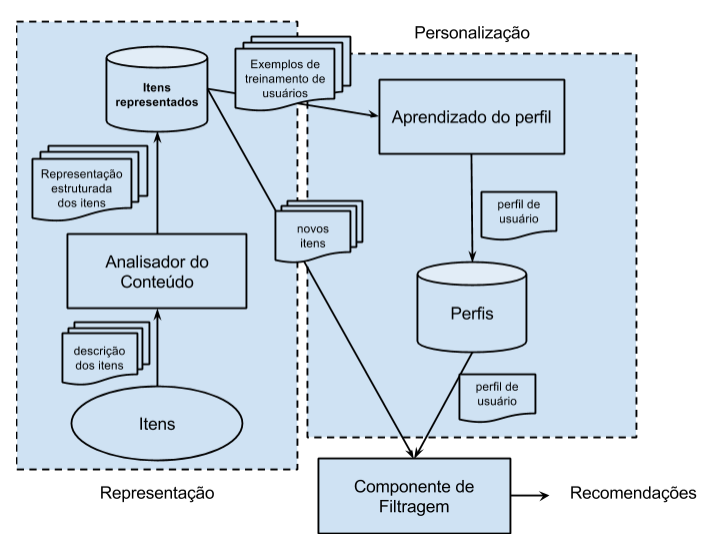
\includegraphics[width=100mm]{img/approach.png}
\caption{Arquitetura de um CBRS}
\label{fig:approach}
\end{figure}

Essa arquitetura apresentada foi adaptada de \cite{Lops2011}, para maior compreendimento e maior adequação com esse trabalho.
As subseções~\ref{subsec:analisadorcontexto},~\ref{subsec:perfil} e~\ref{subsec:filtragem} fazem uma revisão da literatura das técnicas de Aprendizado de Máquina aplicadas aos módulos de um SRbC. 

\subsection{Analisador de Contexto}
\label{subsec:analisadorcontexto}

O Analisador de Contexto tem como função representar o item de uma maneira estruturada, a Figura~\ref{fig:analisador} explica como é construída essa etapa. A entrada são os itens, que são pré-processados, para então aplicar técnicas de Aprendizado de Máquina (Redução de Dimensionalidade ou Tarefas de Aprendizado de Máquina).
Esta etapa compreende o foco deste trabalho.

\begin{figure}[h]
\centering
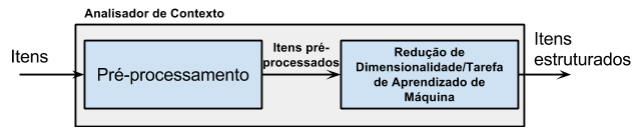
\includegraphics[scale=0.6]{img/analisador}
\caption{Analisador de Contexto.}
\label{fig:analisador}
\end{figure}

Na etapa de pré-processamento, é comum o uso da representação TF-IDF, sendo que existem estudos que propõem outros métodos de representação \cite{Capelle2012, Moerland2013}: SF-IDF (\textit{Semantics Frequency-Inverse Document Frequency}) e SF-IDF+, que obtiveram melhores resultados nos testes apresentados, além disso, \citeonline{Cleger2012} considerou o uso do TF-IDF, mas não resultou em melhores performances.
No entanto, em um SR no contexto de artigos científicos \cite{Beel2013}, foram realizados diversos testes considerando diversos parâmetros e configurações diferentes de representação, resultados mostraram que a configuração com TF-IDF performou melhor que outras.
Outras técnicas de Mineração de Dados também são utilizadas, como \textit{stopwords}, lematização e descarte de termos com frequência abaixo de um limiar.

Na etapa de Redução de Dimensionalidade/Tarefa de Aprendizado de Máquina faz-se o uso extensivo dos algoritmos: LSA (\textit{Latent Semantic Analysis}) \cite{Taraghi2013, Domingues2012, Spaeth2013}, LSI (\textit{Latent Semantic Indexing}) \cite{Saaya2013}, LDA (\textit{Latent Dirichlet Allocation}) \cite{Tantanasiriwong2012, Qu2012, Wang2012, Vaz2012}, que pode ser visto como uma extensão de biclusterização \cite{Skillicorn2012}, e Variáveis Latentes \cite{Cleger2012}, que podem ser vistos por resolver uma tarefa de agrupamento, que é agrupar termos em grupos que são chamados de tópicos \cite{Wang2012}.
O desafio é escolher o número de tópicos, por isso, grande parte dos trabalhos que fazem o uso dessas técnicas, realizam testes variando o número de tópicos.
Esses testes geralmente mostram que esses algoritmos ajudam na performance da recomendação \cite{Cleger2012, Tantanasiriwong2012, Saaya2013, Spaeth2013,Vaz2012}.

Na representação estruturada dos itens, alguns estudos propõem representações no contexto de notícias e artigos científicos \cite{Bielikova2012, Lops2013}: são diferenciadas as relevâncias de cada um dos atributos textuais (exemplo título, conteúdo, categoria e etc.), por meio de pesagem.
Estudos mostraram que com os pesos apropriados é possível melhorar a qualidade da recomendação.
Atributos que não são textuais também são usados no contexto de notícias, como no SR de notícias para celular em \cite{Yeung2012}, que o tempo da notícia modifica o vetor que representa o item, fazendo a multiplicação por um fator $\alpha$. o SR de livros \cite{Vaz2012} que tem como objetivo representar o estilo de escrita de cada autor, faz o uso de atributos como: o tamanho do documento, n-gramas e \textit{vocabulary richness}.

\subsection{Aprendizado do Perfil}
\label{subsec:perfil}

Nesta etapa é onde o perfil do usuário é representado e aprendido pelo SR. Na maioria das vezes o perfil é representado por um vetor de documentos de tamanho $k$, que o usuário visitou ou apresentou um feedback positivo $d_{prefs} = \{d_{pref_1}, d_{pref_2}, \dots, d_{pref_k}\}$.
Há outras formas de representação, como em \citeonline{Yeung2012}, que além da anterior, incorpora informações demográficas, tratando o problema de \textit{user cold-start} em SRsbC.
\citeonline{Vaz2012} propõem uma representação para o perfil do usuário usando um método da área de Recuperação de Informação: algoritmo de \textit{Rocchio}, onde cada documento $d_{pref_i}$ é classificado pelo usuário em positivo ou negativo (como exemplo, gostou ou não gostou), assim o algoritmo faz uma mistura dos exemplos positivos e negativos, com um peso diferente para cada tipo de exemplo, obtendo um vetor.
Então, esse vetor é comparado com vetores de itens (usando similaridade dos cossenos), para obter itens semelhantes.
Variando os parâmetros, os autores chegaram na conclusão que, incorporando exemplos negativos na representação do perfil para treinamento do algoritmo, piora a qualidade das recomendações.

O aprendizado do perfil do usuário é como um problema de classificação, onde o vetor de exemplos é dado por $X = \{d_{pref_i}, y^{+-}_i\}$, sendo que $y^{+-}_i$ representa o rótulo, ou seja, se $d_{pref_i}$ é um item que o usuário gostou($+$) ou não($-$).
Então, é treinado um classificador que irá classificar itens que o usuário ainda não consumiu, para saber se é um item que o usuário irá consumir/gostar.
Diversos algoritmos são usados para resolver esse tipo de problema: Redes Bayesianas \cite{Yeung2012, Cleger2012}, Naïve Bayes \cite{Lee2012, Semeraro2012}, SVM (\textit{Support Vector Machine}) \cite{Tantanasiriwong2012, Lee2012}.

Existem trabalhos que tratam o aprendizado do perfil com técnicas de Aprendizado Semi-Supervisionado, \citeonline{Lee2012} faz uso de comitê de máquinas para construir um modelo de Aprendizado de Máquina que classifica apenas classes positivas, visando classificar se o usuário de um e-commerce irá gostar ou não de um produto. Primeiramente, classifica exemplos sem rótulo, para depois entrarem no modelo final que agrega todos os exemplos (SVM ou Naïve Bayes).
Foi verificado que o SR proposto trata o problema de poucos dados para a identificação do perfil do usuário, pois não necessita apenas de dados rotulados.

É possível tratar o problema de aprendizado do perfil como um problema de clusterização \cite{Davoodi2012, Bielikova2012}.
\citeonline{Davoodi2012} apresentam um SR de especialistas, que representa o perfil dos usuários com semântica e constrói uma \textit{Rede Social}, para então, usar o algoritmo de clusterização (\textit{k-means}) para encontrar perfis de usuário.
Além desse, \cite{Bielikova2012} apresenta um SR de notícias que faz o uso de clusterização hierárquica, tendo como medidade de similaridade a similaridade dos cossenos e índice de jaccard.
Com uma abordagem \textit{bottom-up} de agrupamento e uma estrutura de árvore binária, é realizado a clusterização das notícias: as folhas representam as notícias e os nós pais, clusters que representam temas das notícias.
O usuário desse sistema é representado por caminhos nesta árvore construída, podendo ser recomendados diversas notícias dentro de diversos tópicos, que podem surpreender o usuário, amenizando o problema de serendipidade em SRsbC. 

\subsection{Componente de Filtragem}
\label{subsec:filtragem}

Essa é a etapa mais simples, por ser na maioria das vezes, apenas uma filtragem das recomendações já calculadas na etapa de Aprendizagem do Perfil, essa estratégia é apresentada em \citeonline{Cleger2012, Qu2012, Wang2012, Davoodi2012, Mannens2011, Semeraro2012}. Outra estratégia simples é a determinação de um limiar \cite{Capelle2012, Lops2013}, ou seja, os valores da lista de recomendação gerada são filtradas pelo limiar estabelecido. Nos estudos apresentados, foram encontrados muitos SRs Híbridos, que faziam uma outra abordagem para a filtragem, usando uma combinação dos métodos de Filtro Colaborativo e baseados em conteúdo \cite{Lops2013, Qu2012, Domingues2012, Spaeth2013, Vaz2012}.

O trabalho desenvolvido por \citeonline{Bielikova2012} foi o único que apresentou uma estratégia diferente para o Componente de Filtragem, com a árvore binária montada, todas as notícias dos menores para os maiores grupos, que não foram lidas pelo usuário, foram separadas para a recomendação. Então, é construída uma matriz com as recomendações, sendo as linhas ordenadas pelos grupos menores para os grupos maiores, e as colunas ordenadas pelas notícias mais recentes. Assim, cada coluna é transformada em um vetor, concatenando-os e formando uma lista que é apresentada para o usuário.

\chapter{Proposta}

A proposta desse projeto de mestrado envolve a aplicação de algoritmos de biclusterização para o problema de recomendação baseada em conteúdo textual, a qual, segundo a revisão sistemática que esta sendo realizada, foi muito pouco explorada: apenas um entre $1\;943$ estudos primários relevantes nas bases de dados (não publicado) se refere à aplicação de biclusterização em conteúdo textual.

Com maior especificidade, a proposta desse projeto (Figura~\ref{fig:proposta}) é definida pela utilização de técnicas de mineração de texto para o processamento das notícias presentes no corpus iG (Subseção~\ref{subsec:corpusig}), após a estruturação do texto, serão realizadas diversas representações (TF-IDF, TF-IDF normalizado e n-gramas) para a criação de biclusters com algoritmos de biclusterização, realizando experimentos para verificar a consistência dos biclusters criados pelos diferentes algoritmos aplicados.
Assim, será definida uma estratégia para gerar uma lista de recomendações e comparar com a base de cliques iG (Subseção~\ref{subsec:basecliquesig}), utilizando métricas de SRs para gerar experimentos e avaliar as recomendações geradas. Além disso, será feita uma comparação com um SR do tipo filtro colaborativo, para comparar a \textit{serendipidade} entre o método proposto e o filtro colaborativo.

% redesenhar imagem
\begin{figure}[h]
\centering
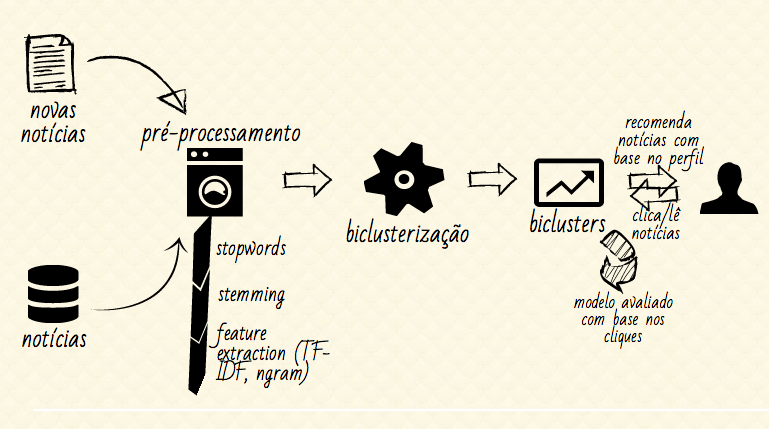
\includegraphics[width=120mm]{img/proposal.png}
\caption{Ilustração da proposta desse mestrado.}
\label{fig:proposta}
\end{figure}

\section{Bases de dados iG}
\label{sec:basesig}

\subsection{Corpus iG}
\label{subsec:corpusig}

O corpus iG, construído neste projeto, é composto por um conjunto de notícias do portal iG\footnote{http://www.ig.com.br/} ${\cal N} = \{ n_1, n_2, \dots, n_m \}$, em que cada notícia $n_i$ é representada pela tupla $(\text{\textit{permalink}}, \text{\textit{título}}, \text{\textit{subtítulo}}, \text{\textit{corpo}}, c_i)$, em que $\text{\textit{permalink}}$ é o endereço eletrônico fixo da notícia, e, $c_i$ um elemento do conjunto de canais $\;{\cal C} = \{ \text{\textit{gente}}, \text{\textit{ultimosegundo}}, \text{\textit{delas}}, \text{\textit{economia}},\\ \text{\textit{esporte}}, \text{\textit{saude}}, \text{\textit{igay}}, \text{\textit{deles}}, \text{\textit{tecnologia}}, \text{\textit{igirl}}, \text{\textit{jovem}}, \text{\textit{arena}}, \text{\textit{luxo}} \}$, onde cada canal representa um assunto ou tópico de notícias.

O número total de notícias do corpus é $m = 4\;593$, com mais de 250 caracteres no corpo, no perído de 02 de Janeiro de 2012 até 11 de Outubro de 2014. As notícias estão bem distribuídas por ano: $1\;551$ notícias em 2012, $1\;933$ notícias em 2013 e $1\;109$ em 2014. Como cada notícia esta associada com um canal, foi coletada a distribuição de notícias por canal (Tabela~\ref{tab:distcanais}).

\begin{table}[h]
\centering
\label{tab:distcanais}
\caption{Distribuição de notícias por canal ($ci$) do corpus iG.}
\begin{tabular}{c|c}
\hline
canal ($ci$)                    & número de notícias \\
\hline
$\text{\textit{gente}}$         & 196 \\
$\text{\textit{ultimosegundo}}$ & 555 \\
$\text{\textit{delas}}$         & 252 \\
$\text{\textit{economia}}$      & 907 \\
$\text{\textit{esporte}}$       & 342 \\
$\text{\textit{saude}}$         & 88  \\
$\text{\textit{igay}}$          & 210 \\
$\text{\textit{deles}}$         & 141 \\
$\text{\textit{tecnologia}}$    & 359 \\
$\text{\textit{igirl}}$         & 527 \\
$\text{\textit{jovem}}$         & 524 \\
$\text{\textit{arena}}$         & 421 \\
$\text{\textit{luxo}}$          & 71  \\
\hline
\end{tabular}
\end{table}

Analisando a distribuição de notícias por ano foi possível verificar que os links escolhidos como partida para o \textit{web crawler} realizar a extração de notícias foram efetivos para deixar a distribuição perto de uniforme, com média e desvio padrão de aproximadamente $1531 \pm 337$ notícias.
Contrariamente, a distribuição de notícias por canal não ficou perto do uniforme, com média e desvio padrão de aproximadamente $353 \pm 225$ notícias, uma hipótese é que isso se deve à idade e popularidade do canal, por exemplo, os canais $\text{\textit{luxo}}$ e $\text{\textit{deles}}$ são muito mais recentes e menos populares que o $\text{\textit{ultimosegundo}}$.

\subsection{Base de cliques iG}
\label{subsec:basecliquesig}

A base de dados de cliques iG, doada para a realização desta pesquisa, é composta por um conjunto usuários anônimos $U = \{ u_1, \dots, u_l \}$ que foram capturados através do controle de cookies dos navegadores do portal, assim, cada usuário $u \in U$ interage com o conjunto de notícias ${\cal N}$ através de cliques, representados por $q_{u,n}^t$, um clique em uma notícia $n$ que foi dado por $u$ em um dado mometo do tempo $t$.
Assim, se considerar cada clique $q_{u,n}^t$ como uma preferência do usuário $u$ por $n$, é possível construir a matriz de preferências $U \times I$ (Seção~\ref{sec:sr}), no contexto, $I = {\cal N}$.

Originalmente a base de cliques iG é composta de $487\;487\;395$ cliques, com $m = xxx$ notícias, coletadas, aproximadamente, do período de abril de 2013 à novembro de 2014. Essa base de dados tem tamanho total, sem compressão, de $100GB$, o que dificulta a sua mineração. No entanto, pretende-se usar apenas as notícias que compõem o corpus iG.

\subsection{Pré-processamento do corpus iG}

O corpus iG, para representar as notícicas de maneira estruturada, foi pré-processado usando algumas técnicas de Mineração de Texto (Seção~\ref{sec:mintexto}).
Foi criado um \textit{pipeline} para o pré-processamento das notícias que contou com as seguintes etapas:
\begin{enumerate}[label*=\arabic*.]
  \item Concatenação das características textuais (título, subtítulo e corpo da notícia) da notícia; normalização do texto, convertendo para minúsculo.
  \item Filtragem de trechos do texto que correspondem com uma lista de expressões regulares definidas através da análise do corpus.
  \item \textit{Tokenização}, usando espaços, pontuações e expressões regulares como delimitadores.
  \item Definição de uma lista de \textit{stopwords}, a partir de uma lista já definida pela biblioteca nltk\footnote{http://www.nltk.org/} (\textit{Natural Language Processing Toolkit}) da linguagem python, foram adicionadas mais \textit{stopwords} à essa lista (por exemplo: \textit{leia mais}, \textit{veja aqui} e etc.), através de uma análise empírica das notícias do corpus.
  \item \textit{Stemming}, para reduzir ambiguidade e a dimensionalidade das notícias, foi aplicado o algoritmo Removedor de Sufixos da Língua Portuguesa (RSLP) Stemmer \cite{Alvares2005}, que leva em consideração a teoria da língua portuguesa para criar 8 etapas, em que, cada etapa é composta por um conjunto de regras e então aplicada uma regra por vez. Este algoritmo é capaz de tratar e remover formas plurais, femininas/masculinas, adverbiais, aumentativas e diminutivas, substantivas, verbais e acentos.
  \item Representação estruturada dos termos em:
  \begin{enumerate}[label*=\arabic*.]
    % \item TF
    \item TF-IDF, realiza a contagem dos termos e aplica a fórmula de TF-IDF.
    \item TF-IDF normalizado, realiza a contagem dos termos, aplica a fórmula de TF-IDF e faz a normalização para que todos os valores fiquem no intervalo de 0 à 1.
    \item \textit{2-grams}, realiza a contagem dos termos concatenando 2 a 2.
    % \item \textit{2-grams TF-IDF}, realiza a contagem dos termos concatenando 2 a 2.
    \item \textit{3-grams}, realiza a contagem dos termos concatenando 3 a 3.
  \end{enumerate}
\end{enumerate}

% \section{Estudos iniciais de biclusterização em conjunto de dados sintéticos} (?)
% \section{Estudos iniciais de biclusterização no corpus IG}

% \textcolor{red}{Texto texto texto texto texto texto texto texto texto texto texto texto texto texto texto texto texto texto texto texto texto texto texto texto texto texto texto texto texto texto texto texto texto texto texto texto texto texto texto texto texto texto texto texto texto texto texto texto texto texto texto texto texto texto texto texto texto texto texto texto texto texto texto texto texto texto texto texto texto texto texto texto texto texto texto.}

% \textcolor{red}{Texto texto texto texto texto texto texto texto texto texto texto texto texto texto texto texto texto texto texto texto texto texto texto texto texto texto texto texto texto texto texto texto texto texto texto texto texto texto texto texto texto texto texto texto texto texto texto texto texto texto texto texto texto texto texto texto texto texto texto texto texto texto texto texto texto texto texto texto texto texto texto texto texto texto texto.}

% \textcolor{red}{Texto texto texto texto texto texto texto texto texto texto texto texto texto texto texto texto texto texto texto texto texto texto texto texto texto texto texto texto texto texto texto texto texto texto texto texto texto texto texto texto texto texto texto texto texto texto texto texto texto texto texto texto texto texto texto texto texto texto texto texto texto texto texto texto texto texto texto texto texto texto texto texto texto texto texto.}

% \textcolor{red}{Texto texto texto texto texto texto texto texto texto texto texto texto texto texto texto texto texto texto texto texto texto texto texto texto texto texto texto texto texto texto texto texto texto texto texto texto texto texto texto texto texto texto texto texto texto texto texto texto texto texto texto texto texto texto texto texto texto texto texto texto texto texto texto texto texto texto texto texto texto texto texto texto texto texto texto.}

\section{Próximos passos - cronograma}

O cronograma apresentado no Gráfico~\ref{misc:cronograma} se refere às atividades a serem desenvolvidas, o progresso indica o que já foi realizado, sendo que as subtarefas já realizadas podem já ter sido completas e não estão indicadas neste cronograma. As tarefas e subtarefas são descritas:
\begin{enumerate}
  \item[{\texttt{[1]}}] Revisão Sistemática de Sistemas de Recomendação baseados em Conteúdo, compreende ao andamento da RS, restando analisar os trabalhos encontrados de 2005 à 2011. Como a RS está sendo feita por 3 pesquisadores, é demandado mais trabalho e, portanto, mais tempo, no entanto, a concentração de trabalhos nos anos mais recentes é maior, significando que a quantidade de trabalho para a realização dessa tarefa não é proporcinal aos anos de abrangência da revisão.
  \begin{enumerate}
    \item[{\texttt{[1.1]}}] Aplicação dos critérios de inclusão e exclusão.
    \item[{\texttt{[1.2]}}] Extração dos resultados.
    \item[{\texttt{[1.3]}}] Elaboração de um artigo, com o intuito de publicação na revista \textit{User Modeling and User-Adapted Interaction}\footnote{\textit{http://www.umuai.org/}} (UMUAI).
  \end{enumerate}
  \item[{\texttt{[2]}}] Estudo de técnicas de Mineração de Texto, como foi necessário o uso de conceitos desta área para a construção do corpus iG, grande parte da literatura necessária já foi levantada e estudada.
  \begin{enumerate}
    \item[{\texttt{[2.1]}}] Estudo de técnicas de pré-processamento de texto.
    \item[{\texttt{[2.2]}}] Estudo de técnicas de redução de dimensionalidade para texto, esta questão foi pouco estudada, e dada a sua importância, será desprendido mais estudos para a mesma.
  \end{enumerate}
  \item[{\texttt{[4]}}] Construção de um corpus de notícias e estruturação do mesmo, como o corpus já foi construído, esta tarefa já esta $95\%$ completa.
  \begin{enumerate}
    \item[{\texttt{[3.1]}}] Implementação de técnicas de pré-processamento de texto.
    \item[{\texttt{[3.2]}}] Implementação de técnicas de representação de texto.
  \end{enumerate}
  \item[{\texttt{[4]}}] Estudo e aplicação de técnicas de Biclusterização.
  \begin{enumerate}
    \item[{\texttt{[3.1]}}] Estudo das técnicas de Biclusterização, incluindo algoritmos e formas de avaliação.
    \item[{\texttt{[3.2]}}] Implementação das técnicas e algoritmos de Biclusterização, um dos algoritmos estudados já foi implementado \cite{Cheng2000} e esta disponibilizado em \textit{https://github.com/lucasbrunialti/biclustering-experiments}.
    \item[{\texttt{[3.3]}}] Validação das técnicas implementadas em conjuntos de dados sintéticos, o algoritmo implementado já foi testado em conjuntos de dados sintéticos, possibilitando a aprendizagem do seu comportamento.
    \item[{\texttt{[3.4]}}] Aplicação dos algoritmos no corpus iG.
  \end{enumerate}
  \item[{\texttt{[5]}}] Análise dos resultados obtidos pelas estratégias propostas e implementadas.
  \begin{enumerate}
    \item[{\texttt{[5.1]}}] Avaliação através de medidas internas de biclusterização.
    \item[{\texttt{[5.2]}}] Avaliação através de medidas externas de biclusterização, como a informação dos canais presentes no corpus iG e a base de dados de cliques iG.
  \end{enumerate}
  \item[{\texttt{[6]}}] Escrita da dissertação.
\end{enumerate}

\noindent
\begin{ganttchart}[
    vgrid,
    hgrid,
    x unit=4.5mm,
  ]{1}{33}
  \label{misc:cronograma}
  \gantttitle{Jan}{3}
  \gantttitle{Fev}{3}
  \gantttitle{Mar}{3}
  \gantttitle{Abr}{3}
  \gantttitle{Mai}{3}
  \gantttitle{Jun}{3}
  \gantttitle{Jul}{3}
  \gantttitle{Ago}{3}
  \gantttitle{Set}{3}
  \gantttitle{Out}{3}
  \gantttitle{Nov}{3} \\

  \ganttgroup[progress=40]{[1]}{1}{9} \\
  \ganttbar[progress=30]{[1.1]}{1}{6} \\
  \ganttbar[progress=10]{[1.2]}{3}{8} \\
  \ganttbar[progress=5]{[1.3]}{1}{9} \\

  \ganttgroup[progress=80]{[2]}{1}{7.5} \\
  \ganttbar[progress=95]{[2.1]}{1}{1.5} \\
  \ganttbar[progress=20]{[2.2]}{2}{4} \\

  \ganttgroup[progress=95]{[3]}{1}{3} \\
  \ganttbar[progress=100]{[3.1]}{1}{3} \\
  \ganttbar[progress=80]{[3.2]}{2}{3} \\

  \ganttgroup[progress=15]{[4]}{1}{27} \\
  \ganttbar[progress=45]{[4.1]}{1}{24} \\
  \ganttbar[progress=20]{[4.2]}{1}{21} \\
  \ganttbar[progress=20]{[4.3]}{2}{24} \\
  \ganttbar[progress=00]{[4.4]}{6}{27} \\

  \ganttgroup[progress=0]{[5]}{19}{27} \\
  \ganttbar[progress=00]{[5.1]}{19}{27} \\
  \ganttbar[progress=00]{[5.2]}{19}{27} \\

  \ganttgroup[progress=0]{[6]}{4}{33}
\end{ganttchart}

%  \item Análise dos resultados obtidos pelas estratégias propostas.
%      medidas internas de bicluster
%      medidas externas (canais, base de cliques)
    
% ********** REFERÊNCIAS **********

%\bibliography{abnt-options,abnt-10520-2001,abnt-10520-2002,abnt-6023-2000,normas,abnt-test,abntex-doc,dissertacao}

\bibliography{refs}                 % o nome do arquivo .bib com as referências

%***********************************
%***** Anexos e Apêndices *********
%***********************************


\end{document}
